















\chapter{Validated Automatic Brain Extraction of Head CT Images}
\label{chap:ss}


\section{Introduction}

X-ray computed tomography (CT) scanning of the brain is widely available and is a commonly used diagnostic tool in clinical settings \citep{sahni_management_2007, chalela2007magnetic, schellinger1999standardized}. Though analysis of CT images is typically done by qualitative visual inspection, detailed quantification of information using neuroimaging tools is of interest.  The reason for this interest is that qualitative inspection of CT scans provides limited quantifiable information that can be used in research. A fundamental processing step for producing quantifiable and  reproducible information about the brain is to extract the brain from the CT image. This process is called brain extraction or skull stripping.  This step is necessary because CT images contain non-brain human tissues and non-human elements (e.g. pillow, medical devices) that are not pertinent to brain research.  We propose a validated automated solution to brain extraction in head CT scans using established neuroimaging software.

In magnetic resonance imaging (MRI), brain extraction has been extensively studied and investigated (see \citet{wang2014knowledge} for an overview of methods).  While an extensive literature accompanied by software exist for brain MRI scans, the same is not true for brain CT scans.  \citet{smith_fast_2002} introduced and validated the Brain Extraction Tool (BET), a function of the FSL \citep{jenkinson_fsl_2012} neuroimaging software (v5.0.4), to automatically extract the brain from MRI scans.  Here we propose to adapt BET and validate its brain extraction performance for CT scans.  

BET adaptations for this purpose have been presented before in \citet{solomon_user-friendly_2007}.  Although the method is similar to that outlined below, using thresholding and then applying BET, the authors did not publish the specific details of the method nor any code to evaluate it.  To replicate the method from \citet{solomon_user-friendly_2007}, \citet{rorden_age-specific_2012} thresholded voxels to be under 100 Hounsfield units, manually adjusted the image intensity to enhance the soft tissue in the brain, and then BET was applied with a fractional intensity of $0.35$.  Therefore, brain extraction methods from \citet{rorden_age-specific_2012} and \citet{solomon_user-friendly_2007} strongly parallels the proposed method described below, but neither studies presented a formal validation against a set of manually segmented brain images.  

\citet{mandell2014volumetric1} has recently proposed a brain extraction method for CT scans and has done a validation against manual segmentation.  This method was also performed on a set of brains with disease \citep{mandell2014volumetric2, mandell2014volumetric3}.  This method is not fully automated, however.   \citet{mandell2014volumetric1} has formally validated a brain extraction method against manually segmented images, but the method requires user interaction.  

Thus, the goals of our study are to propose an automated method that has been formally validated against a set of manually segmented images and estimate brain extraction performance of this method in a large number of CT scans.





\section{Methods}
\subsection{ Participants and CT data}
We used CT images from patients enrolled in the MISTIE (Minimally Invasive Surgery plus recombinant-tissue plasminogen activator for Intracerebral Evacuation) and ICES (Intraoperative CT-Guided Endoscopic Surgery) stroke trials \citep{morgan_preliminary_2008}.  Inclusion criteria into the study included: $18$ to $80$ years of age, spontaneous supratentorial intracerebral hemorrhage above $20$ milliliters (mL) in size (for full criteria, see \citet{mould_minimally_2013}).  The population analyzed here had a mean (SD) age was $60.6$ $(11.6)$ years, was $66.9\%$ male, and was 55.6\% Caucasian, 30.1\% African American, 9.8\% Hispanic, and 4.5\% Asian or Pacific islander.  CT data were collected as part of the Johns Hopkins Medicine IRB-approved MISTIE research studies with written consent from participants.  


\subsection{Imaging Data}
\subsubsection{Validation of Automated Head Segmentation}
For the validation of automated segmentation against gold standard manual segmentation, we analyzed 36 scans, corresponding to 36 unique patients.  The study protocol was executed with minor, but important, differences across the 19 sites.  Scans were acquired using Siemens ($N=14$), GE ($N=11$), Philips ($N=10$), and Toshiba ($N=1$) scanners. Gantry tilt was observed in 21 scans.  Slice thickness of the image varied within the scan for 7 scans. For example, a scan may have 10 millimeter (mm) slices at the top and bottom of the brain and 5mm slices in the middle of the brain.  Therefore, the scans analyzed had different voxel (volume element) dimensions and image resolution prior to registration to the template.  These conditions represent how scans are presented for evaluation in many diagnostic cases.  

%n_crani_problem 
%n_gantry_problem 


\subsection{Manual and Automated Brain Extraction}
Brain tissue was manually segmented as a binary mask from DICOM (Digital Imaging and Communications in Medicine) images using the OsiriX imaging software (OsiriX v.4.1, Pixmeo; Geneva, Switzerland) by one expert reader (reader 1: NU). 
CT brain images and the binary brain tissue mask obtained using manual segmentation were exported from OsiriX to DICOM format.  

\subsection{Image Processing}
The image processing pipeline is provided in Figure~\ref{fig:framework}.
Images with gantry tilt were corrected using a customized MATLAB (The Mathworks, Natick, Massachusetts, USA) user-written script (\url{http://bit.ly/1ltIM8c}).  Although gantry tilt correction is not inherently necessary for brain extraction, it is required for rigid co-registration of scans within a patient, which is a common processing step in longitudinal analysis of images post brain extraction. 

Images were converted to the Neuroimaging Informatics Technology Initiative (NIfTI) data format using \texttt{dcm2nii} (2009 version, provided with MRIcro \citep{rorden_stereotaxic_2000}).  Images were constrained to values between $-1024$ and $3071$ HU to remove potential image rescaling errors and artifacts.  No interpolation was done for images with a variable slice thickness. Thickness was determined from the first converted slice and the NIfTI format assumes homogeneous thickness throughout the image.  This loss of information, if not properly accounted for, affects volume estimation, which relies on accurate pixel dimensions in millimeters.  Variable slice thickness should have no affect on the other estimates of performance described below as they are calculated at a voxel level and do not rely on pixel resolution.  Although the NIfTI images store the data with only one pixel dimension for the height of the voxel, we use the ImagePositionPatient DICOM field to determine the accurate height of each voxel to calculate an accurate volume.  


\tikzstyle{bblock} = [rectangle, draw, text width=8em, text centered, minimum height=2em, rounded corners]
\tikzstyle{line} = [draw, text centered , -latex']
\tikzstyle{line node} = [draw, fill=white, font=\tiny ]
\tikzstyle{block} = [rectangle, draw, text width=5em, text centered, minimum height=4em, rounded corners]    

\begin{figure}
\centering
\begin{tikzpicture}[node distance = 2cm, every node/.style={rectangle,fill=white}, scale=0.75, transform shape]
% Place nodes
\node [bblock] (raw) {DICOM images};
\node [bblock, below = 2.5cm of raw] (dcmnii) {NIfTI image};
\node [bblock, below of=dcmnii] (thresh) {Threshold to 0-100 HU };
\node [bblock, above right=1cm and 1.25cm of dcmnii] (gantry) {Gantry tilt correction};
\node [bblock, below of=thresh, left of=thresh] (nosmooth) {No Smooth};
\node [bblock, below of=thresh, right of=thresh] (smooth) {Smooth ($1$mm$^3$)};

\node [bblock, below of=nosmooth, right of=nosmooth] (BET) {BET};

\node [block, below of=BET, node distance = 3cm] (SS_1) {FI=0.1};
\node [block, left = 1.75em of SS_1] (SS_01) {FI=0.01};
\node [block, right = 1.75em of SS_1] (SS_35) {FI=0.35};

\node [block, below of=SS_1] (Mask) {Threshold image $> 0$ (Mask)};

\node [block, below of=Mask, node distance = 2cm] (Fillin) {Fill mask holes};

\node [bblock, below of=Fillin, node distance = 2cm] (Measures) {Performance Measures};


% Draw edges
\path [line] (raw) -- node {dcm2nii} (dcmnii);
\path [line] (raw) -- (gantry);
\path [line] (gantry) -- node {dcm2nii} (dcmnii);
\path [line] (dcmnii) -- (thresh);
\path [line] (thresh) -- (nosmooth);
\path [line] (thresh) -- (smooth);
\path [line] (smooth) -- (BET);
\path [line] (nosmooth) -- node[above right= -0.15cm and -0.6cm of BET] {Threshold $0-100$ HU} (BET);
\path [line] (BET) -- (SS_01);
\path [line] (BET) -- (SS_35);
\path [line] (BET) -- node {Different fractional intensity (FI) Value} (SS_1);
\path [line] (SS_1) -- (Mask);
\path [line] (SS_01) -- (Mask);
\path [line] (SS_35) -- (Mask);
\path [line] (Mask) -- (Fillin);
\path [line] (Fillin) -- (Measures);
\end{tikzpicture}
\caption[{\bf Brain Extraction Processing Pipeline.}]{{\bf Brain Extraction Processing Pipeline.}  Images in DICOM (Digital Imaging and Communications in Medicine) format were gantry tilt corrected if necessary and converted to NIfTI (Neuroimaging Informatics Technology Initiative) format using \texttt{dcm2nii}.  After NIfTI conversion, the data is thresholded to tissue ranges of $0-100$ Hounsfield units (HU).  In one variant of the pipeline, the data was smoothed using a 3-dimensional Gaussian kernel ($\sigma=1$mm$^3$) and re-thresholded to $0-100$ HU; in the other, the data was not smoothed.  BET was applied to the image using 3 different fractional intensity (FI) values: $0.01$, $0.1$, and $0.35$.  The resultant image was masked to values greater than $0$ HU and FSL was used to fill in any holes.  These filled masks were used in comparison to the manually segmented image.  }
\label{fig:framework}
\end{figure}

Each image was thresholded using the brain tissue range ($0-100$ HU); voxels outside this range were set to $0$ HU.  In one variant of the pipeline, data were smoothed using a 3-dimensional (3D) Gaussian kernel ($\sigma=1$mm$^3$) and re-thresholded to $0-100$ HU; in the other, data were not smoothed.  BET was then applied, varying the fractional intensity (FI) parameter to determine its influence on performance: we used values of $0.35$ (as used in \citet{rorden_age-specific_2012}), $0.1$, and $0.01$.  

The FI parameter varies between $0$ and $1$ and determines the location of the edge of the segmented brain image; smaller values correspond to larger brain masks. \citet{smith_fast_2002} describes that the FI parameter determines a local threshold $t_{l}$ by the following equation:
$$
t_{l} = \left(I_{\text{max}} - t_2\right) \times \text{FI} + t_2
$$
where $I_{\text{max}}$ is a local maximum intensity along a line from an outer surface vertex pointing inward to the image center and $t_2$ is the $2^{nd}$ percentile of the image distribution.  As a result of thresholding in our pipeline, $t_2$ equals $0$ HU and $I_{\text{max}}$ must lie between $0$ and $100$ HU.  Therefore, after thresholding,
$$
t_{l} = I_{\text{max}} \times \text{FI}.
$$
With an $I_{\text{max}}$ of $100$ HU, using an FI lower than $0.01$ results in $t_{l}$ less than $1$ HU, but greater than $0$ HU.  As CT data is stored as integers, no intensities lie between $0$ and $1$, so a $t_{l}$ between $0$ or $1$ HU should provide similar local thresholds.  Therefore, we chose $0.01$ as a lower limit for testing FI. 


After BET was applied, we created a brain mask taking values $> 0$ HU and filled the holes in the mask (using \verb|fslmaths -fillh|).  


\subsection{Measuring and Testing Brain Extraction Performance}
We compared the masks obtained using the various choices of parameters to the manually segmented images.  Four common measurements of performance were calculated for each image: sensitivity, specificity, accuracy, and the Dice Similarity Index (DSI) \citep{dice_measures_1945}.  For each measure, higher values indicate better agreement with the manual segmentation.  See Inline Supplementary Methods 1 for the calculation of each measure.

[Insert Supplementary Methods 1 here]

We calculated the paired difference of each measure using different pipelines (e.g. $0.01$ vs. $0.1$, smoothed data).  We tested whether these differences were statistically different from zero using the Wilcoxon signed-rank test.

From each scan, we also calculated the intracranial volume (ICV), defined as all voxels inside the skull, by multiplying the number of voxels in the resulting mask by the dimensions of each voxel.  We calculated the ICV ratio comparing manual and automated segmentation: $\frac{\text{ICV}_{\text{automated}}}{\text{ICV}_{\text{manual}}}$.  A ratio of $1$ indicates the same volume; greater than $1$ indicates over-estimation of ICV; less than $1$ indicates underestimation of ICV.  As adjustment for ICV has been shown to reduce inter-subject variation in volumetric studies \citep{whitwell2001normalization}, we wish to estimate ICV accurately. 


\subsection{Consistency of Manual Brain Extraction}
As manual segmentation can have intra-reader variability, another reader (reader 2: AM) manually segmented brain tissue on the 36 scans.  We additionally estimated all four performance measurements, using the manual segmentation from reader 2 as the gold standard.  We also estimated the ICV from the segmentation from reader 2.   We calculated the ICV ratio $\left(\frac{\text{ICV}_{\text{reader 2}}}{\text{ICV}_{\text{reader 1}}}\right)$ and the correlation of ICV estimates across readers.

\subsection{Failure Rate and Intraclass Correlation Estimate}
Although comparison of automated methods to a manual gold standard is ideal, manual segmentation requires a significant amount of time.  Therefore, for a large number of scans, this procedure is impractical.  As multiple CT scans are obtained from patients in the MISTIE trial, we can estimate the reliability of our proposed brain extraction pipelines without manual segmentation by comparing intracranial volumes of the same patient on subsequent scans.  Moreover, we can estimate failure rate of each pipeline.  

For these tasks, we collected 1160 scans.  Of these scans, we excluded 27 scans due to craniotomy and 38 due to the gantry tilt correction forcing areas of the brain outside the field of view.   We executed the previous brain extraction pipelines on the remaining 1095 scans.  Of these scans, we visually assessed the quality of brain extraction: any scan excluding a significant portion of the brain or having holes due to mask self-intersection were classified as a failure.  These scans represent 129 patients from 26 sites, with a mean (SD) of 8.5 (2.8) scans per patient.  Scans were acquired using Siemens ($N=492$), GE ($N=298$), Philips ($N=207$), Toshiba ($N=66$), Neurologica ($N=30$), and Picker ($N=2$) scanners.  We estimated the failure rate for each processing pipeline and used a Fisher's exact test to test whether failure rates differed across scanners.


For each scan, we calculated the ICV.  Using only the scans with successful brain extraction, we estimated the intraclass correlation (ICC) and its confidence interval (CI) of ICV using a one-way ANOVA, where a patients was treated as a group, for unbalanced repeated measures \citep{searle_linear_2012, thomas_interval_1978, donner_use_1979, lessells_unrepeatable_1987} using the ICC package \citep{wolak_guidelines_2012} in R (\url{http://cran.r-project.org/}).  
%and the Jaccard index is defined as:
%$$
%\frac{ \sum_{i=1}^{V} \left( I_{ia} \times I_{im}\right) }{\sum_{i=1}^{V} I_{ia}  + \sum_{i=1}^{V} I_{im} - \sum_{i=1}^{V} \left(I_{ia} \times I_{im} \right)}
%$$



\section{Results}
\subsection{Manual and Automated Brain Extraction}
The following estimates use the manual segmentation from reader 1 as the gold standard. Figure~\ref{fig:metrics}\protect\subref*{unsmoothed} illustrates the performance of each variation of the BET pipeline in Figure~\ref{fig:framework}.  The pipelines using smoothing (top panel) perform better than the unsmoothed pipelines (bottom panel) on all measures except specificity (all $p < 0.01$, uncorrected for multiplicity).  BET also performed poorly on some scans without smoothing.  

Figure~\ref{fig:metrics}\protect\subref*{smoothed} displays the performance for brain extraction for the pipelines using smoothed images.   Because the performance for all metrics was high when using smoothed images, it was necessary to change the y-axis from $[0,1]$ to $[0.95,1]$. 
Using an FI of $0.01$ or $0.1$ performed better than $0.35$; thus, we will focus and compare results for these values of FI only for the case when BET was applied to smoothed images.  Using an FI of $0.01$ had a higher median sensitivity ($0.9901$) than an FI of $0.1$ ($0.9884$, median difference: $0.0014$, $p< 0.001$), accuracy ($0.9971$ vs. $0.9971$; median difference: $0.0001$, $p< 0.001$), and DSI ($0.9895$ vs. $0.9894$; median difference: $0.0004$, $p< 0.001$) and lower specificity ($0.9981$ vs. $0.9982$; median difference: $-0.0001$, $p< 0.001$).  Overall, regardless of p-values, these measures are all very high, indicating that multiple choices of parameters work well for brain extraction after CT image processing.  Moreover, a Bonferroni correction for multiple comparisons yields the same conclusions. 

The mean (SD) ICV ratio was $1.002$ ($0.0079$) using an FI of $0.01$ and $1$ ($0.0081$) using an FI of $0.1$.  Both mean ratios are close to $1$ with a small variance, indicating the ICV estimates are similar for automated and manual segmentation. 

The above results indicate that using smoothed data and an FI of $0.01$ or $0.1$ had high performance when compared to the manual segmentation of reader 1.  The results were similar using the scan-wise union of the segmentation from reader 1 and reader 2.  Using the manual segmentation from reader 2 or the scan-wise intersection of the segmentation from reader 1 and reader 2, the median values using and $0.1$ had higher marginally performance than using $0.01$ for DSI, accuracy, and specificity, but lower performance for sensitivity.  See Inline Supplementary Figure 1 for the distribution of performance metrics for each segmentation.

[Inline Supplementary Figure 1]

Regardless of which manual segmentation was used, estimates of performance for each scan using smoothed data and an FI of $0.01$ or $0.1$ remained above $0.95$.  Thus, these pipelines perform well, yet one FI may not perform universally better than the other.  

% Overall, using an FI of $0.35$ performs worse overall than $0.01$ or $0.1$ for all measures other than specificity.  
% 
% Without smoothing the images, BET performed poorly regardless of FI.  
% 












\begin{figure}
  \subfloat{
  \label{unsmoothed}
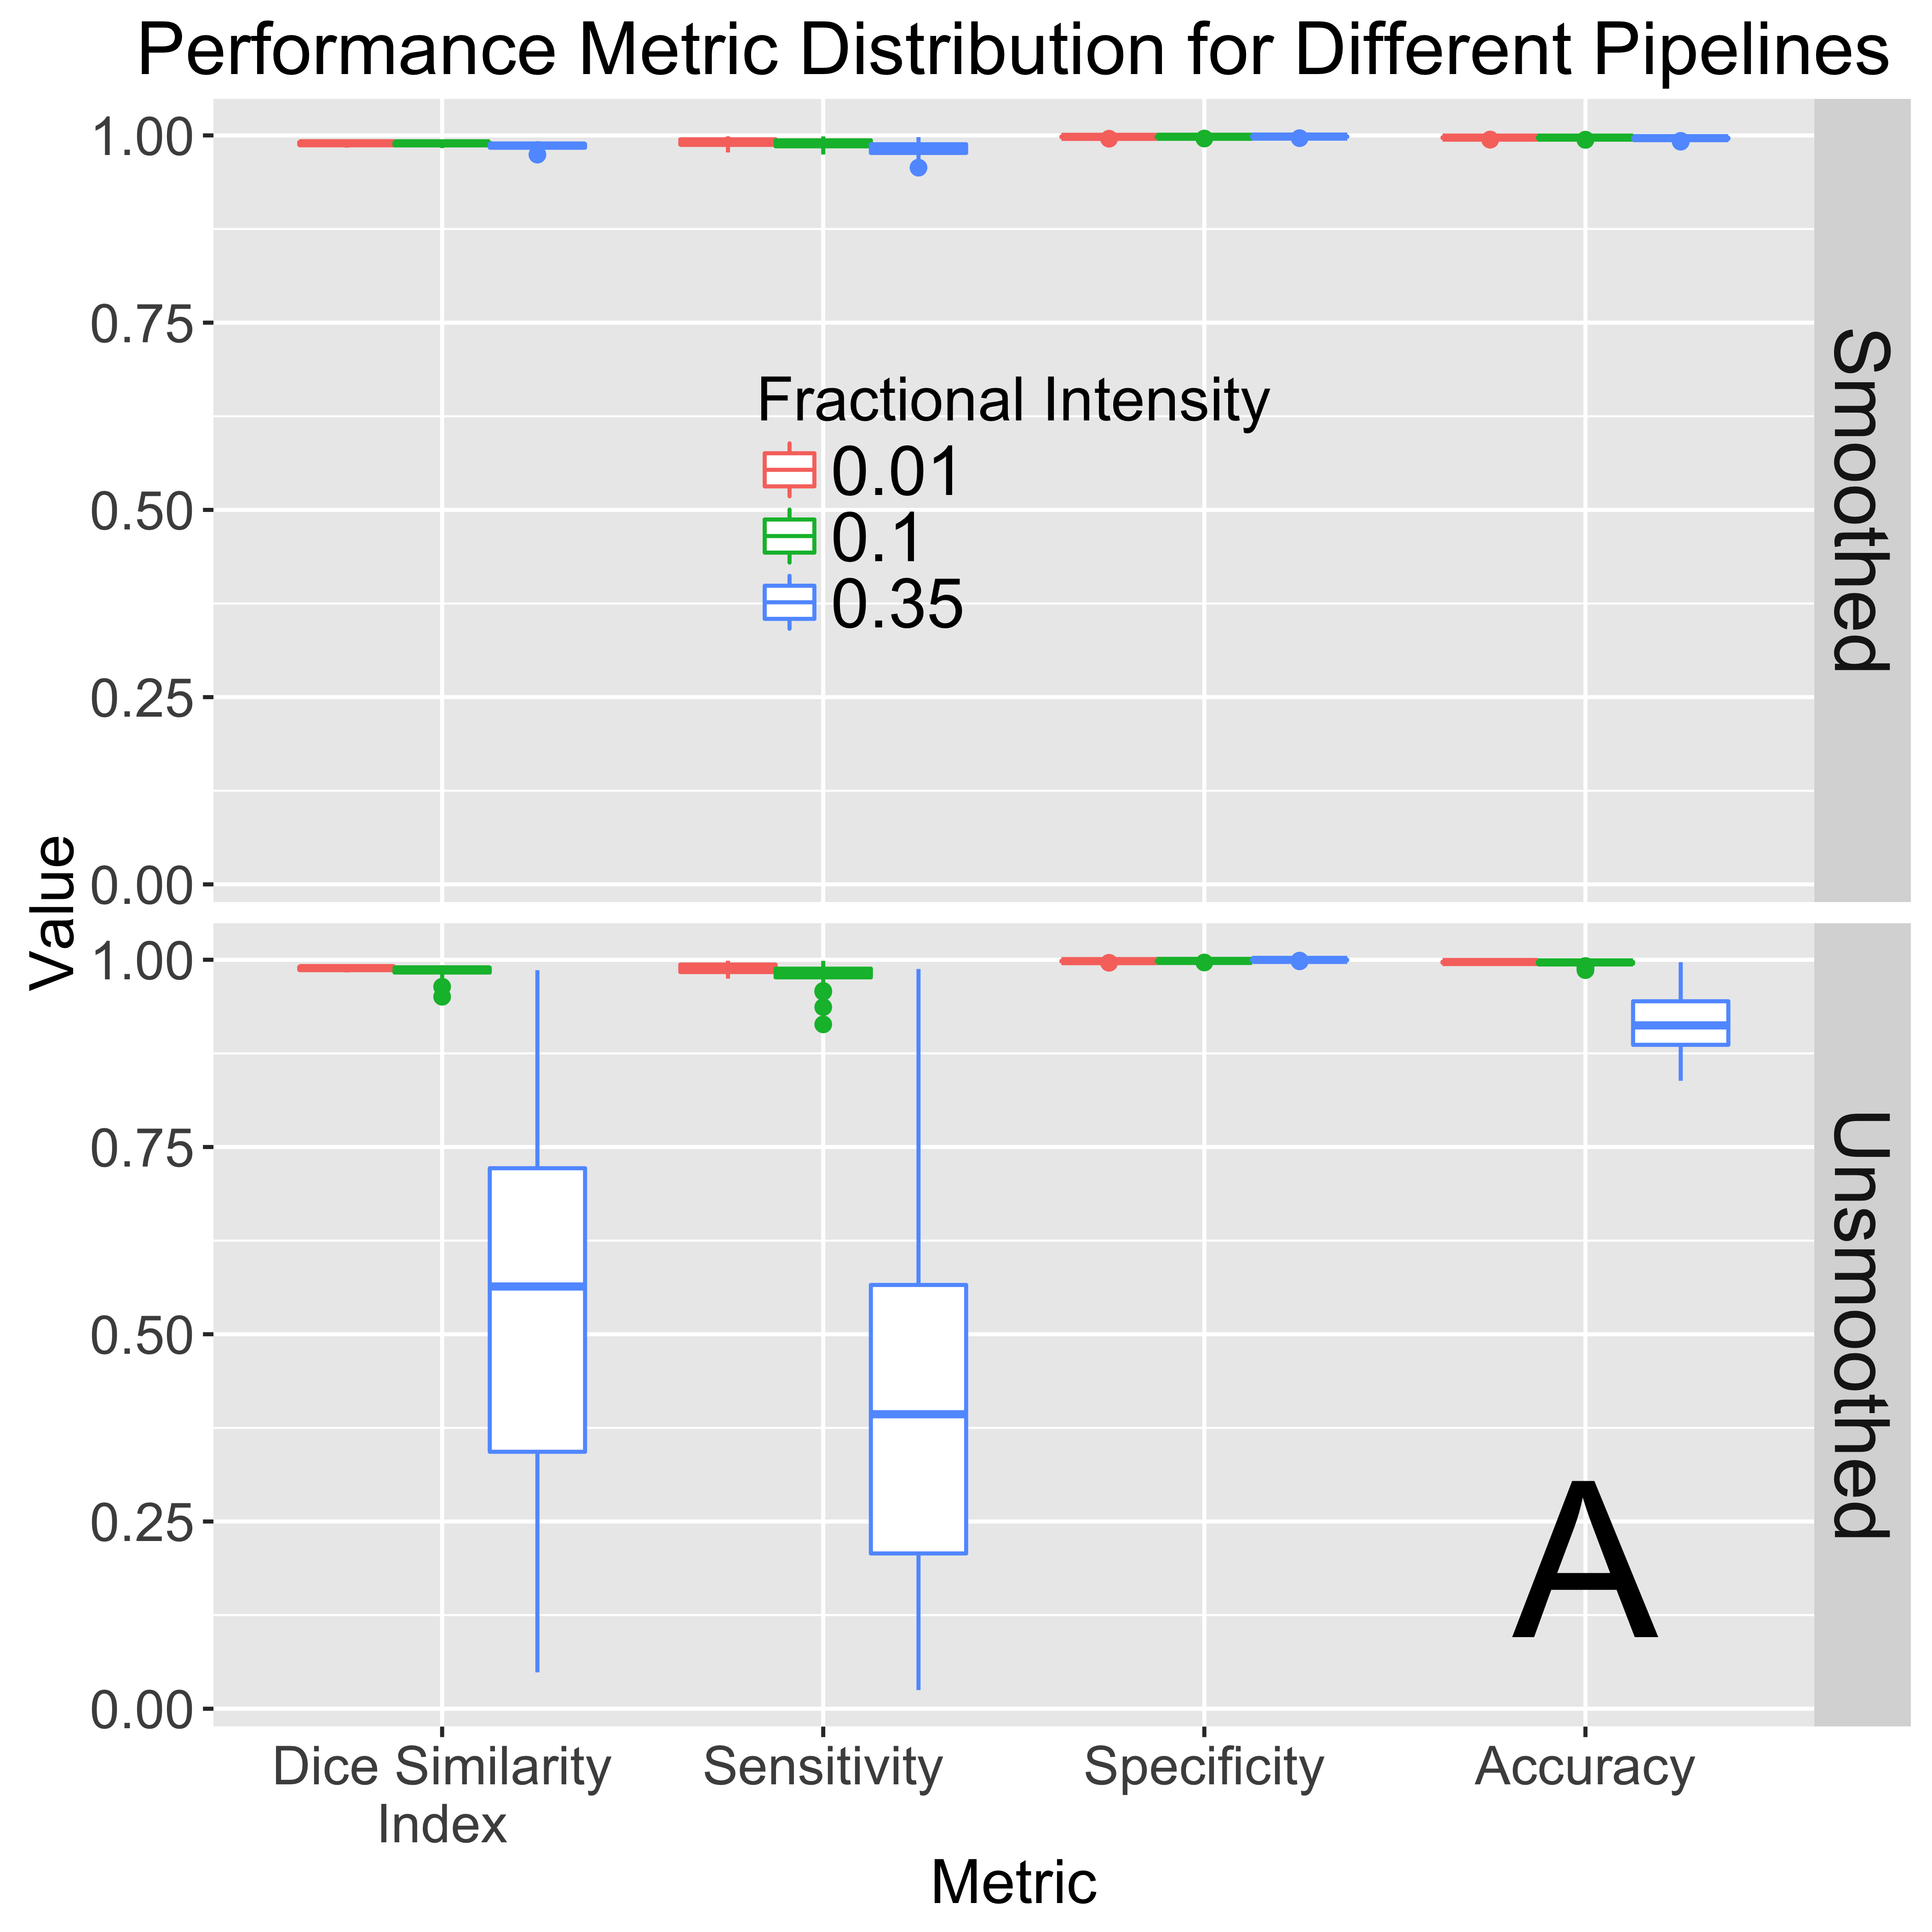
\includegraphics[width=.48\textwidth]{figure/CT_Skull_Stripping_Figure2.png}
}
\hfill
  \subfloat{
  \label{smoothed}
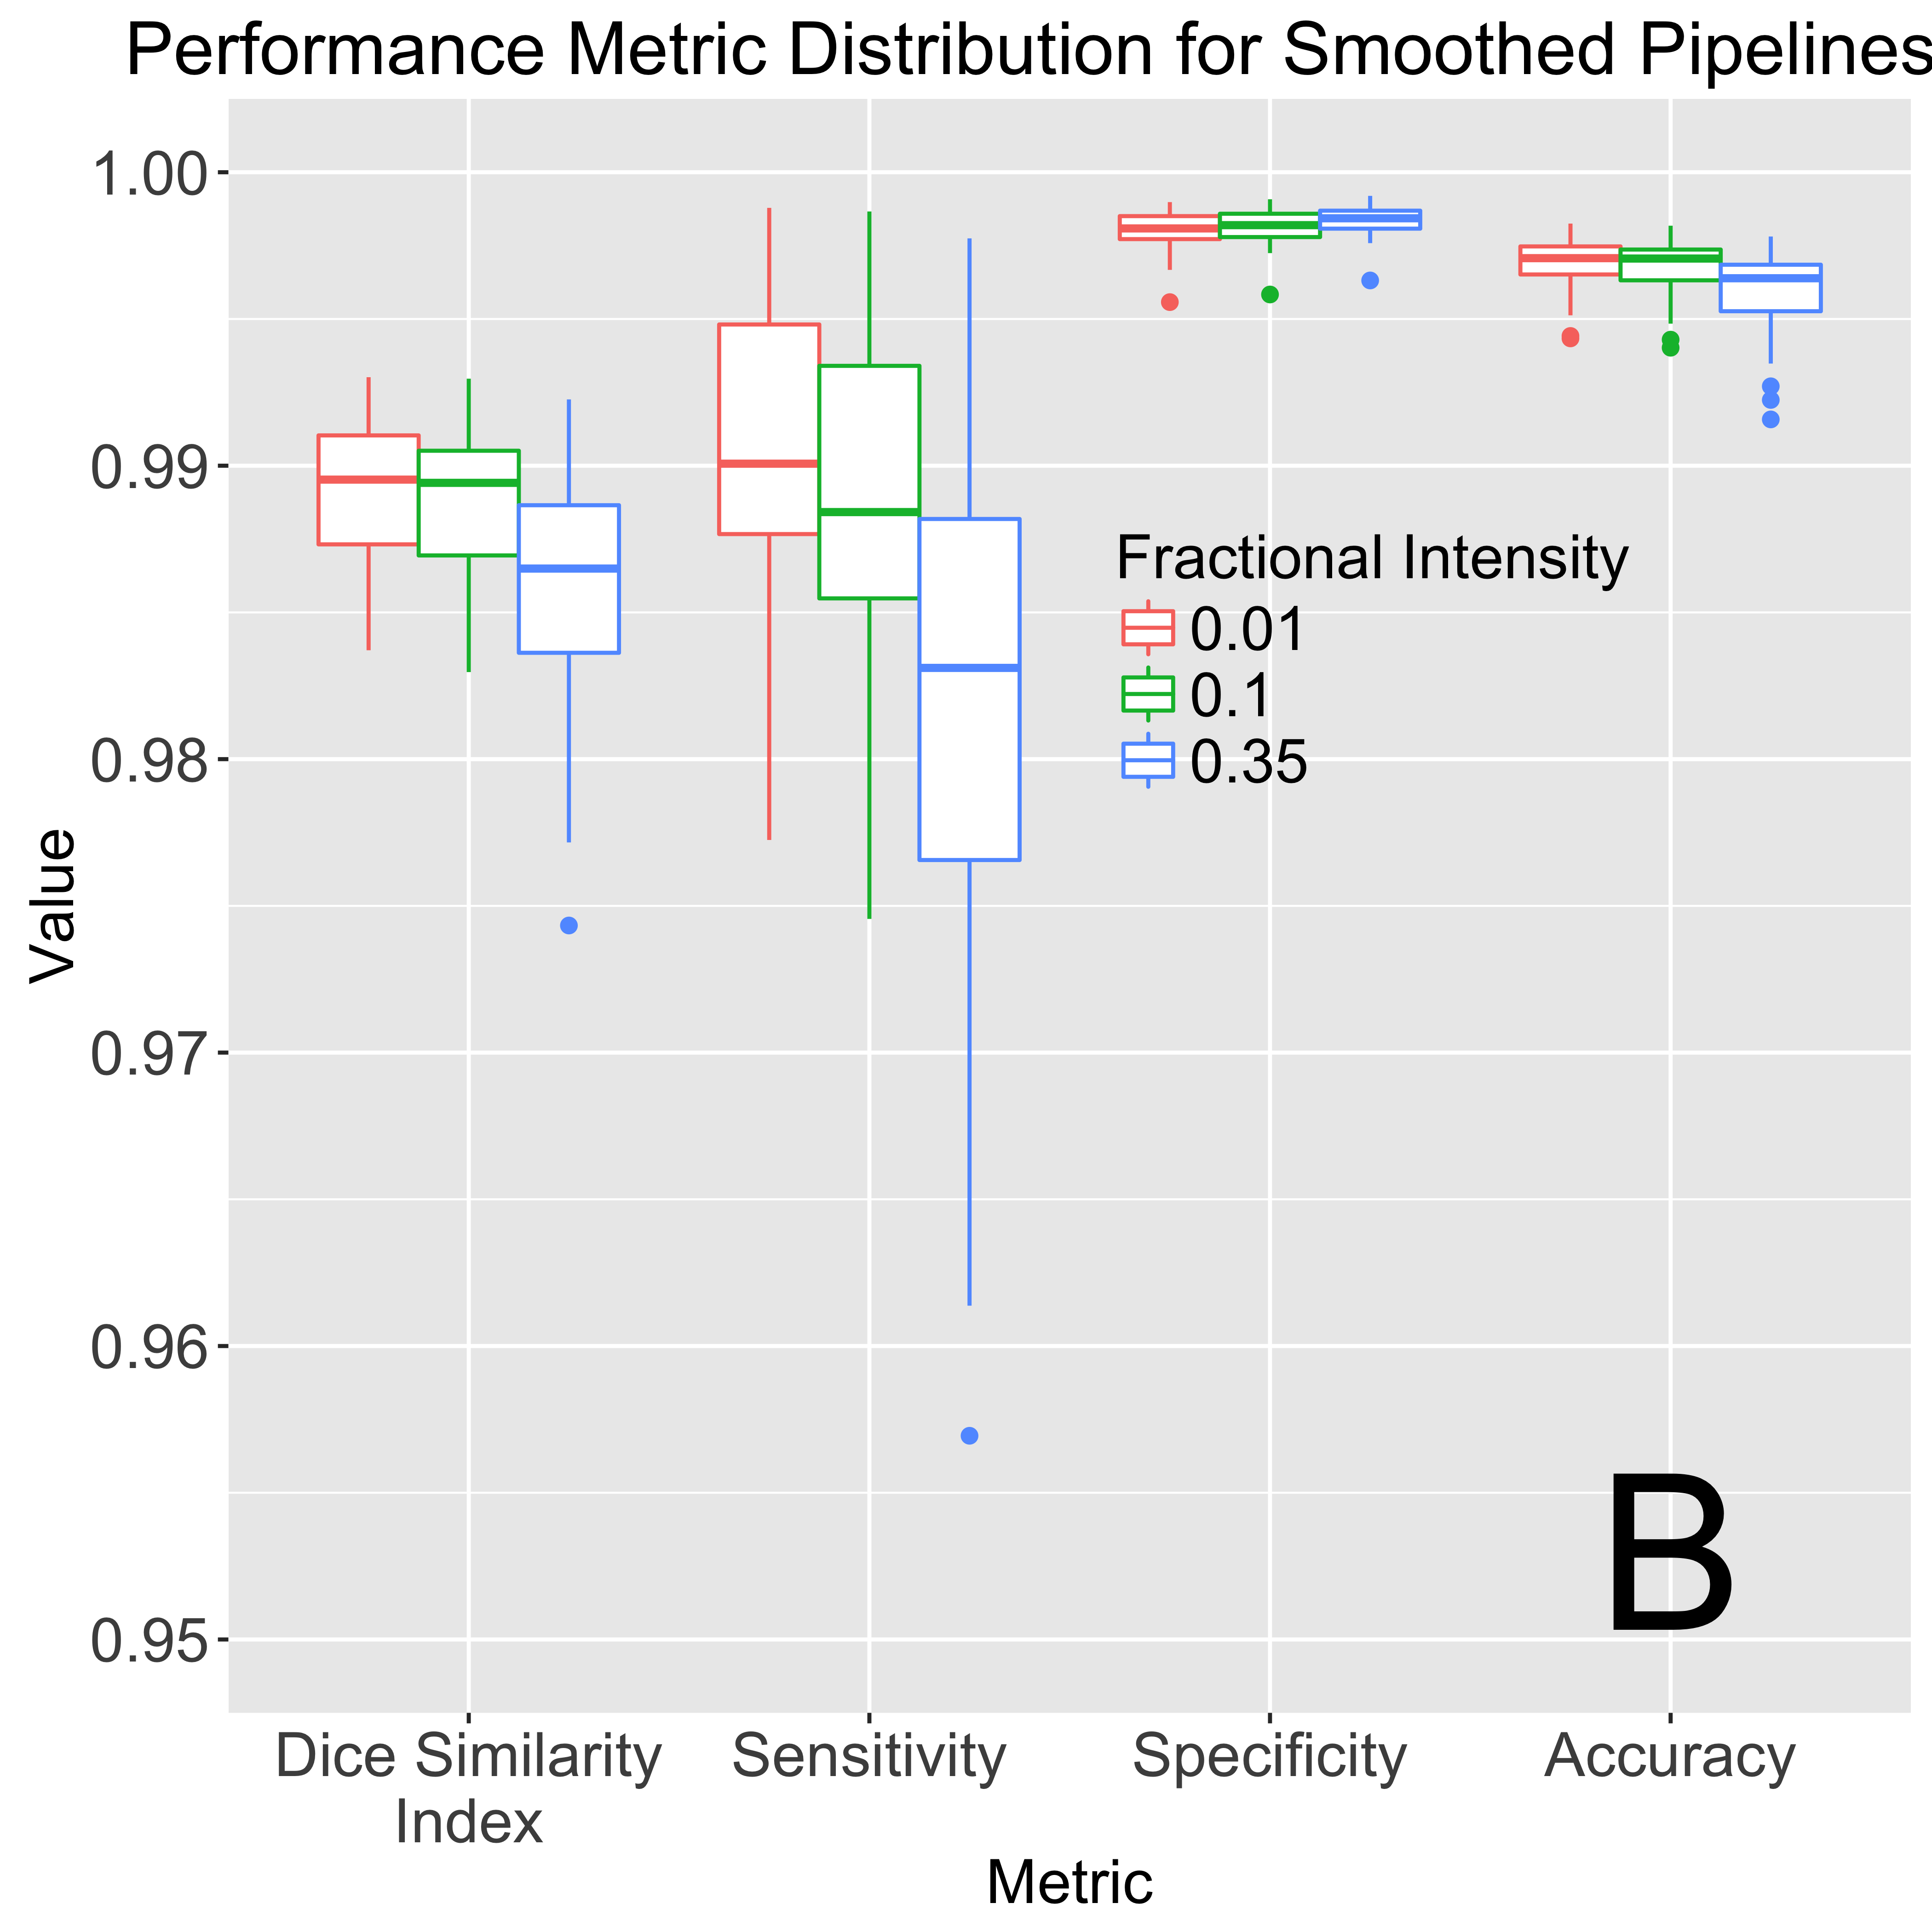
\includegraphics[width=.48\textwidth]{figure/CT_Skull_Stripping_Figure2b.png}
}
\caption[{\bf Performance Metric Distribution for Different Pipelines.}]{{\bf Performance Metric Distribution for Different Pipelines.} Panel~\protect\subref*{unsmoothed} displays the boxplots for performance measures when running the pipeline with a different fractional intensity (FI), using smoothed data (top) or unsmoothed data (bottom).  Panel~\protect\subref*{smoothed} presents the smoothed data only, rescaled to show discrimination between the different FI. Overall, FI of $0.01$ and $0.1$ perform better than $0.35$ in all categories other than specificity.  Using smoothed data improves performance in all performance metrics, markedly when an FI of $0.35$ is used.  Panel~\protect\subref*{smoothed} demonstrates that using an FI of $0.01$ on smoothed data has high performance on all measures.  }
\label{fig:metrics}
\end{figure}



\begin{figure}[htb]
\centering
  \subfloat{
  \label{ss:01_smooth}
	\includegraphics[width=.315\textwidth]{figure/{101-307_20061110_1638_CT_5_RM_Head_SS_0.01_Mask}.png} 
}
\hfill
  \subfloat{
  \label{ss:1_smooth}
	\includegraphics[width=.315\textwidth]{figure/{101-307_20061110_1638_CT_5_RM_Head_SS_0.1_Mask}.png} 
}
\hfill
  \subfloat{
  \label{ss:35_smooth}
	\includegraphics[width=.315\textwidth]{figure/{101-307_20061110_1638_CT_5_RM_Head_SS_0.35_Mask}.png} 
}
\newline
\hfill 
  \subfloat{
  \label{ss:01_nosmooth}
	\includegraphics[width=.315\textwidth]{figure/{101-307_20061110_1638_CT_5_RM_Head_SS_0.01_nopresmooth_Mask}.png} 
}
\hfill
  \subfloat{
  \label{ss:1_nosmooth}
	\includegraphics[width=.315\textwidth]{figure/{101-307_20061110_1638_CT_5_RM_Head_SS_0.1_nopresmooth_Mask}.png} 
}
\hfill
  \subfloat{
  \label{ss:35_nosmooth}
	\includegraphics[width=.315\textwidth]{figure/{101-307_20061110_1638_CT_5_RM_Head_SS_0.35_nopresmooth_Mask}.png} 
}
\caption[{\bf Example Case where Smoothing before BET is Required.}]{{\bf Example Case where Smoothing before BET is Required.} For one subject, the CT image is displayed with the brain extracted mask in red after running all pipelines.  Panels~\protect\subref*{ss:01_smooth}, \protect\subref*{ss:1_smooth}, and \protect\subref*{ss:35_smooth} represent applying BET using FI of $0.01$, $0.1$, and $0.35$, respectively, to smoothed data. Panels~\protect\subref*{ss:01_nosmooth}, \protect\subref*{ss:1_nosmooth}, and \protect\subref*{ss:35_nosmooth} correspond to applying BET using FI $0.01$, $0.1$, and $0.35$ on unsmoothed data.  Smoothing images improves brain extraction with BET.
}
\label{fig:ss_example}
\end{figure}



\subsection{Consistency of Manual Brain Extraction}
%The mean (95\% Confidence Interval (CI)) was $ests['dice', 'mean']$ ($ests['dice', 'lower'], ests['dice', 'upper']$) for DSI, $ests['accur', 'mean']$ ($ests['accur', 'lower'], ests['accur', 'upper']$) for accuracy, $ests['sens', 'mean']$ ($ests['sens', 'lower'], ests['sens', 'upper']$) for sensitivity, and $ests['spec', 'mean']$ ($ests['spec', 'lower'], ests['spec', 'upper']$) for specificity.  The estimated mean (95\% CI) ratio of the ICV was $ests['ratio', 'mean']$ ($ests['ratio', 'lower'], ests['ratio', 'upper']$). 

When comparing manual segmentations, we used the manual segmentation from reader 1 as the gold standard and the segmentation from reader 2 as the test segmentation similar to the automated segmentation above.  The mean (SD) was $0.989$ ($0.0030$) for DSI, $0.997$ ($0.0010$) for accuracy, $0.982$ ($0.0060$) for sensitivity, and $0.999$ ($0.0003$) for specificity.  

The estimated mean (SD) ratio of the ICV was $0.988$ ($0.0068$).  The correlation (95\% confidence interval) of ICV was $0.998$ ($0.997, 0.999$).  See Inline Supplementary Figure 2 for the comparison of ICV estimates from reader 1 and reader 2.

[Inline Supplementary Figure 2]


Overall, we observe high agreement of segmentation between raters and the estimates of performance in automated segmentation to be similar to multiple reader segmentation.  Differences between manual segmentation occurred on the boundary between bone and non-bone areas towards the surface of the cortex and inferior regions of the brain, where one may or may not classify areas as spinal cord and not part of the brain stem.  Thus, the difference observed in the performance of FI of $0.01$ compared to $0.1$ when using a reader 2 as the gold standard are likely due to these areas.  


\subsection{Failure Rate and Intraclass Correlation Estimate}
Although Figure~\ref{fig:metrics} indicates that using FI of $0.01$ or $0.1$ provides adequate brain extraction results for the cases analyzed, they perform relatively well regardless whether or not the data are smoothed.  Figure~\ref{fig:ss_example} displays an example where using unsmoothed data performs poorly for these FIs, demonstrating why smoothing may be necessary for some scans.  This is a high-resolution scan, with voxel size 0.49mm$\times$0.49mm$\times$1, which may result in more noise in the image that may affect the performance of BET.  Moreover, in Table~\ref{tab:fail}, the estimated failure rates were lower using the smoothed data compared to the unsmoothed data.  We observe the lowest failure rate in the pipelines using smoothed data and an FI of $0.01$ or $0.1$.  Though this represents a large number of scans, failure rates may also be affected by patient-level characteristics, including the center where the patient was scanned.  

% latex table generated in R 3.2.2 by xtable 1.8-0 package
% Fri Jan 29 01:56:41 2016
\begin{table}[ht]
\centering
\begin{tabular}{cr|r}
  \hline & \multicolumn{2}{c}{Failure Scans: N (\%)} \\Fractional Intensity & Unsmoothed & Smoothed \\ 
  \hline
0.01 & 161 (14.7\%) & 57 (5.2\%) \\ 
  0.1 & 192 (17.5\%) & 80 (7.3\%) \\ 
  0.35 & 1068 (97.5\%) & 154 (14.1\%) \\ 
   \hline
\end{tabular}
\caption{{\bf Failure Rates for each Processing Pipeline of Brain Extraction of the 1095 Scans Analyzed.}} 
\label{tab:fail}
\end{table}


As multiple scanners were used, we wanted to determine if the failure rate was different across scanners.  In Table~\ref{tab:sfail}, we present the failure rate for each scanner, using smoothed data and an FI of $0.01$.  The failure rates for all scanner types other than Neurologica were below $6\%$.  Although we see a failure rate above $16\%$ in the Neurologica scanners, only $30$ scans were acquired using this type of scanner.  Moreover, a Fisher's exact test did not find a difference in the failure rates across scanner type ($p=0.110$).

% latex table generated in R 3.2.2 by xtable 1.8-0 package
% Fri Jan 29 01:56:41 2016
\begin{table}[ht]
\centering
\begin{tabular}{cc}
 Scanner Type & Failure Rate: Fail/N (\%) \\ 
  \hline
Siemens & 28/492 (5.7\%) \\ 
  GE & 15/298 (5.0\%) \\ 
  Philips & 7/207 (3.4\%) \\ 
  Toshiba & 2/66 (3.0\%) \\ 
  Neurologica & 5/30 (16.7\%) \\ 
  Picker & 0/2 (0.0\%) \\ 
   \hline
\end{tabular}
\caption{{\bf Failure Rates for Different Scanner Types using Smoothed Data and an FI of $0.01$ Processing Pipeline of Brain Extraction of the 1095 Scans Analyzed.}} 
\label{tab:sfail}
\end{table}


The ICC estimate was high using the successfully brain extracted scans from the smoothed data with an FI of $0.01$ (ICC: 0.929, 95\% CI: 0.91, 0.945) and $0.1$ (ICC: 0.928, 95\% CI: 0.909, 0.944).  In Figure~\ref{fig:icc}, we illustrate the ICV estimates, using an FI of $0.01$ and smoothed data, for successful brain extraction in scans 10 or fewer days post baseline scan (gray lines).  The black lines represent ICV estimates over time for $10$ randomly selected patients.  The blue line is a local regression (LOESS) \citep{cleveland_local_1992} line, which represents an estimate of the average ICV over time.  This LOESS line is relatively flat, indicating that the ICV estimate averaged over patients is stable.  We also observe that although within-patient variability exists for ICV estimates, the variability across patients is greater.  

\begin{figure}[htbp]
\centering
\includegraphics[width=.55\textwidth]{figure/{Intraclass_Correlation_no_crani_check_day10_black_0.01_truevol}.png}
\caption[{\bf Intracranial Volume (ICV) Estimates for Scans Less than 10 Days Post-Baseline.}]{{\bf Intracranial Volume (ICV) Estimates for Scans Less than 10 Days Post-Baseline.} These estimates are from the brain extraction pipeline using and FI of $0.01$ and smoothed data.  Each separate line represents an individual patient.  The black lines represent ICV estimates over time for $10$ randomly selected patients.  The blue line is a local regression (LOESS) scatterplot smoother.  
}
\label{fig:icc}
\end{figure}




\section{Discussion}
Quantitative procedures based on data contained in head CT images require brain-only images for analysis. We have introduced the first validated, fully automated brain extraction pipeline for head CT images based on widely used, existing software. Validation was done using gold-standard manual segmentations of brain tissue and multiple measurements of intracranial volume per patient.  A novel finding is that smoothing the data, as opposed to other studies which have smoothed at other points in the process \citep{mandell2014volumetric1}, using a conservative smoother ($1$mm$^3$ 3D Gaussian kernel) and using an FI of $0.01$ or $0.1$ provides good brain extraction for the sample studied.  These choices make a large difference in the performance of the algorithms and have not been previously reported in the literature.

Although the sample size was relatively small for the gold standard validation, the CT images used are from different people, different centers, and different scanners.  We have also shown that failure rates are low (5\%) using smoothed data and an FI of $0.01$ in a large number of scans.  
We are using a population of patients with intracranial hemorrhage and the accuracy of BET may be dependent on factors such as hematoma size, which may change the distribution of Hounsfield units or compress brain structures.  We observed good performance of BET in these patients using the parameters described, which may indicate even better performance for individuals with no observed pathology.  BET also performs well in scans from follow-up scans with no hemorrhage included in the longitudinal ICV estimates; these scans should be more similar to scans from patients without hemorrhage.   

We did not, however, rigorously test this pipeline against a set of different levels of noise (as was done using MRI in \citep{mandell2014volumetric1}), convolution filters, scanning artifacts, or scanning parameters.  As noted in \citet{mandell2014volumetric1}, there is no standard ground truth for CT scans.  However, as these scans are those presented for evaluation in many diagnostic cases, we believe these do represent clinically relevant scans that would be analyzed.  As the failure rates are low, we believe this method may be adapted for different settings of acquisition for CT.  

A percentage of scans in this study did not have successful brain extraction, however.  Additional steps may be done to decrease the failure rate of the proposed method: 1) using registration to a CT template \citep{rorden_age-specific_2012} to remove slices of the neck below the head can achieve better brain-center estimation used by BET; 2) performing BET using a higher smoothness constraint that may reduce potential holes in the brain mask caused by mask intersection; and 3) using a dilation followed by an erosion operation to fill any holes that are caused by thresholding but not filled by the hole filling operation above.  


One additional concern is how general this method is to other populations as the data is from an older adult population, such as the pediatric population \citep{mandell2014volumetric2} analyzed.   \citet{gousias2008automatic} analyzed 33 2-year-old children who had been born prematurely and found that after preprocessing of co-registration and neck removal, and dilation, BET was adequate for brain extraction in MR images, and then brain labeling.  Moreover, \citet{shi2012label} demonstrated BET performed well in automated brain extraction for pediatric MR images of neonates < 2 months ($N = 90$), 1-2 year infants ($N = 141$) and 5-18 year old children ($N = 60$).  Although CT scans may have differences compared to MRI, we believe this method should be robust at least to children, but would like to validate our method on additional populations.  

Overall, good performance using CT acquired under different scanners and different scanning parameters indicate that the approach described here will likely generalize in addition to the fact that CT scan data are expressed in standardized units (Hounsfield units).  Moreover, the robust success of BET as a method is another indicator that our proposed method has a high likelihood of generalizability.


After creating an accurate brain mask, secondary image processing or estimation steps can be performed.  These include intensity normalization, segmentation, and image registration.  Moreover, ICV estimates can be used as potential factor for adjustment in analysis \citep{whitwell2001normalization}.  Additionally, extraction of structures within the brain, such the cerebrospinal fluid (CSF), which can be estimated from the method described in \citet{volkau2010ventricle}, may have fewer errors if performed on the segmented image as the process is not computed over voxels outside of the brain.  We believe that successful brain extraction is fundamental for calculating quantitative measures on the brain and performing necessary secondary operations required for analysis.

%

The research presented here is fully reproducible and we provide ready-to-use software for CT brain extraction. The R function designed to perform brain extraction is located at
\url{http://bit.ly/CTBET_RCODE} and example bash script for command-line FSL can be downloaded here \url{http://bit.ly/CTBET_BASH}.  As our software is publicly available and is based on open-source, free programs (FSL and R), the proposed method is readily available to all users.

\section*{Acknowledgements}
We thank the patients and families who volunteered for this study and Genentech Inc. for the donation of the study drug (Alteplase).

\section*{Sources of Funding}
The project described was supported by the NIH grant RO1EB012547 from the National Institute of Biomedical Imaging And Bioengineering, T32AG000247 from the National Institute on Aging, R01NS046309, RO1NS060910, RO1NS085211, R01NS046309, U01NS080824 and U01NS062851 from the National Institute of Neurological Disorders and Stroke, and RO1MH095836 from the National Institute of Mental Health. Minimally Invasive Surgery and rt-PA in ICH Evacuation Phase II (MISTIE II) was supported by grants R01NS046309 and U01NS062851 awarded to Dr. Daniel Hanley from the National Institutes of Health (NIH)/National Institute of Neurological Disorders and Stroke (NINDS).  ICES was led by Co-Principal Investigator Dr. Paul Vespa at the University of California Los Angeles. Minimally Invasive Surgery and rt-PA in ICH Evacuation Phase III (MISTIE III) is supported by the grant U01 NS080824 awarded to Dr. Daniel Hanley from the National Institutes of Health (NIH)/National Institute of Neurological Disorders and Stroke (NINDS). Clot Lysis: Evaluating Accelerated Resolution of Intraventricular Hemorrhage Phase III (CLEAR III) is supported by the grant U01 NS062851 awarded to Dr. Daniel Hanley from the National Institutes of Health (NIH)/National Institute of Neurological Disorders and Stroke (NINDS). 

\newpage
\section*{Inline Supplementary Methods 1}
Let $I_{ia}, I_{im}$ be the indicators that voxel $i$ is labeled to be in the brain mask for the automatic and manual masks, respectively.  

A voxel $i$ is labeled to be a true positive (TP) when $I_{ia} = 1$ and $I_{im} = 1$, false positive (FP) when $I_{ia} = 1$ and $I_{im} = 0$, false negative (FN) when $I_{ia} = 0$ and $I_{im} = 1$, and true negative (TN) when $I_{ia} = 0$ and $I_{im} = 0$.  Let the total number of voxels be denoted by $V$.  The number of true positive voxels is defined as: 
$$
\# \text{TP} = \sum_{i=1}^{V} \left( I_{ia} \times I_{im}\right)
$$
Sensitivity is defined as
$$
\frac{\# \text{TP} }{\# \text{TP} + \text{FN}} = \frac{ \sum_{i=1}^{V} \left( I_{ia} \times I_{im}\right) }{ \sum_{i=1}^{V} I_{im}},
$$
specificity is defined as
$$
\frac{\# \text{TN} }{\# \text{TN} + \text{FP}} = \frac{ \sum_{i=1}^{V} \left\{ (1-I_{ia}) \times (1- I_{im} ) \right\} }{ \sum_{i=1}^{V} (1 - I_{im} )},
$$
overall accuracy is defined as:
$$
\frac{\# \text{TN} + \text{TP} }{\# \text{TN} + \text{FN} + \text{TP} + \text{FP}} = \frac{ \sum_{i=1}^{V} \left[ (I_{ia} \times I_{im}) + \left\{ (1-I_{ia}) \times (1- I_{im} ) \right\} \right] }{ V },
$$
and the Dice Similarity Index (DSI) is defined as
$$
\frac{2 \times \#\text{TP} }{ \# \text{TP} + \text{FN} + \text{TP} + \text{FP}} = \frac{ 2 \times \sum_{i=1}^{V} \left( I_{ia} \times I_{im}\right) }{\sum_{i=1}^{V} I_{ia}  + \sum_{i=1}^{V} I_{im}}.
$$

\section*{Inline Supplementary Figure 1}
\begin{figure}[H]
  \subfloat{
  \label{reader2}
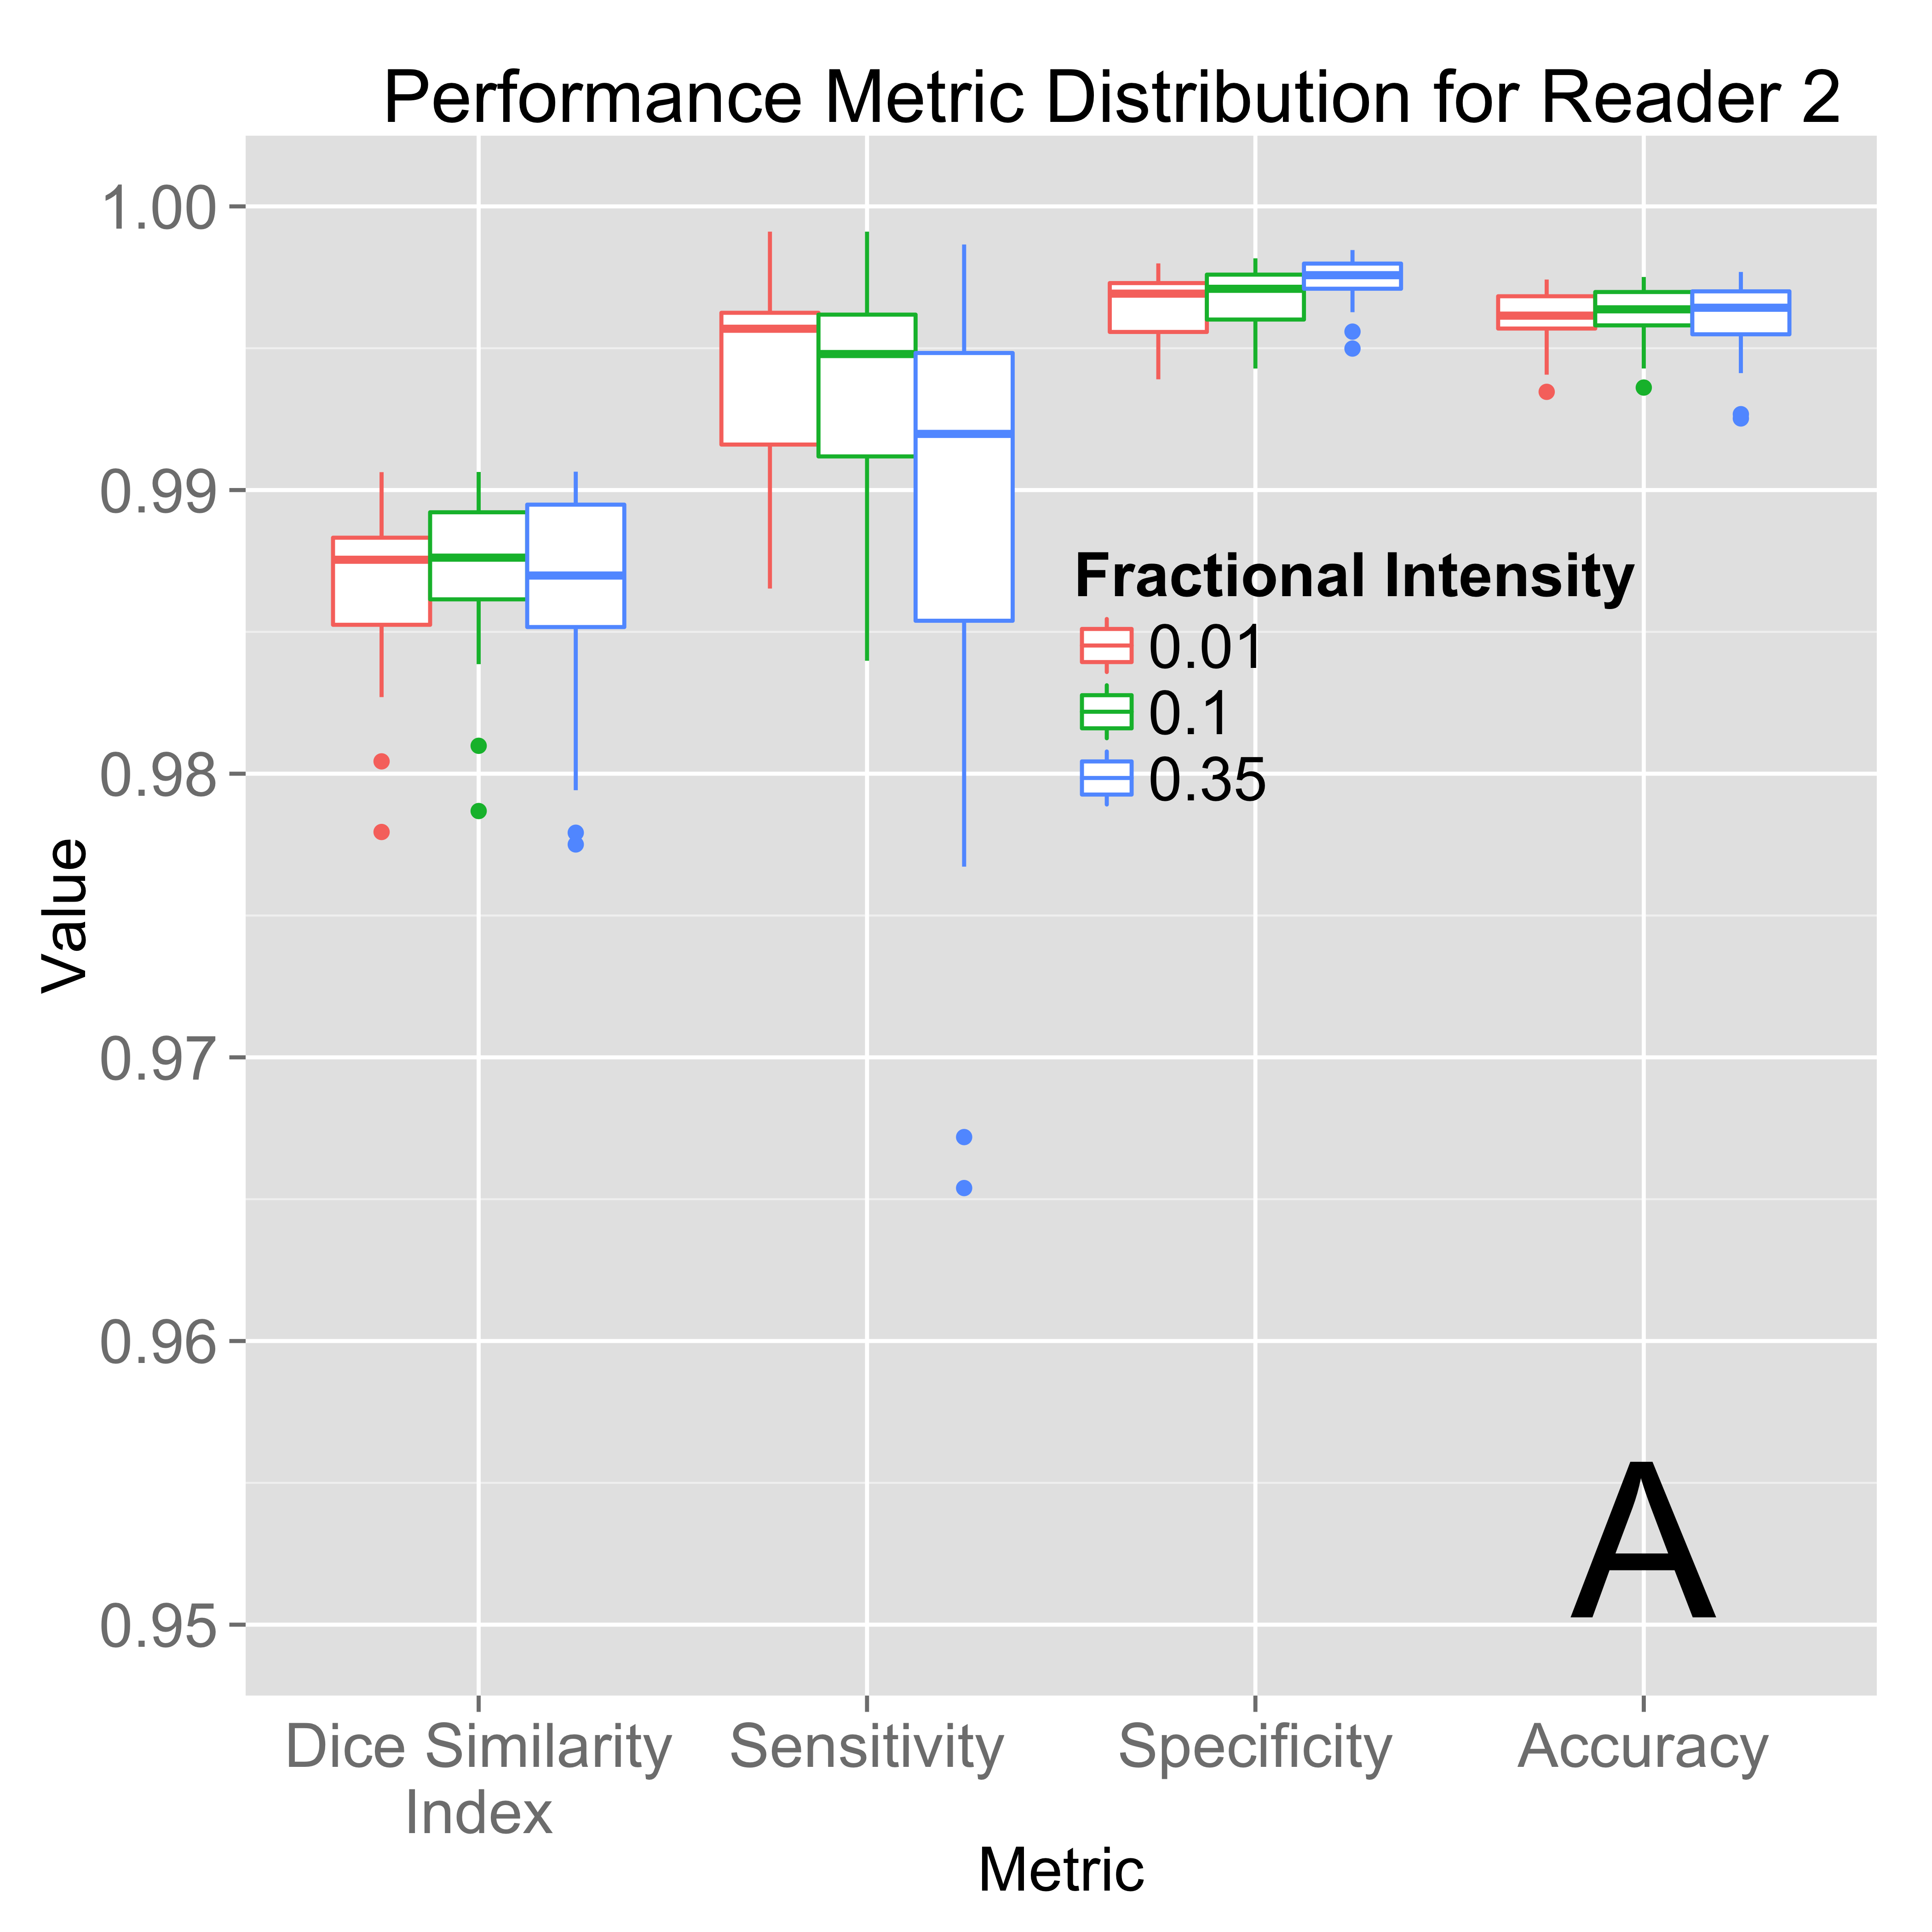
\includegraphics[width=.315\textwidth]{figure/AM_CT_Skull_Stripping_Figure2b.png}
}
\hfill
  \subfloat{
  \label{intersect}
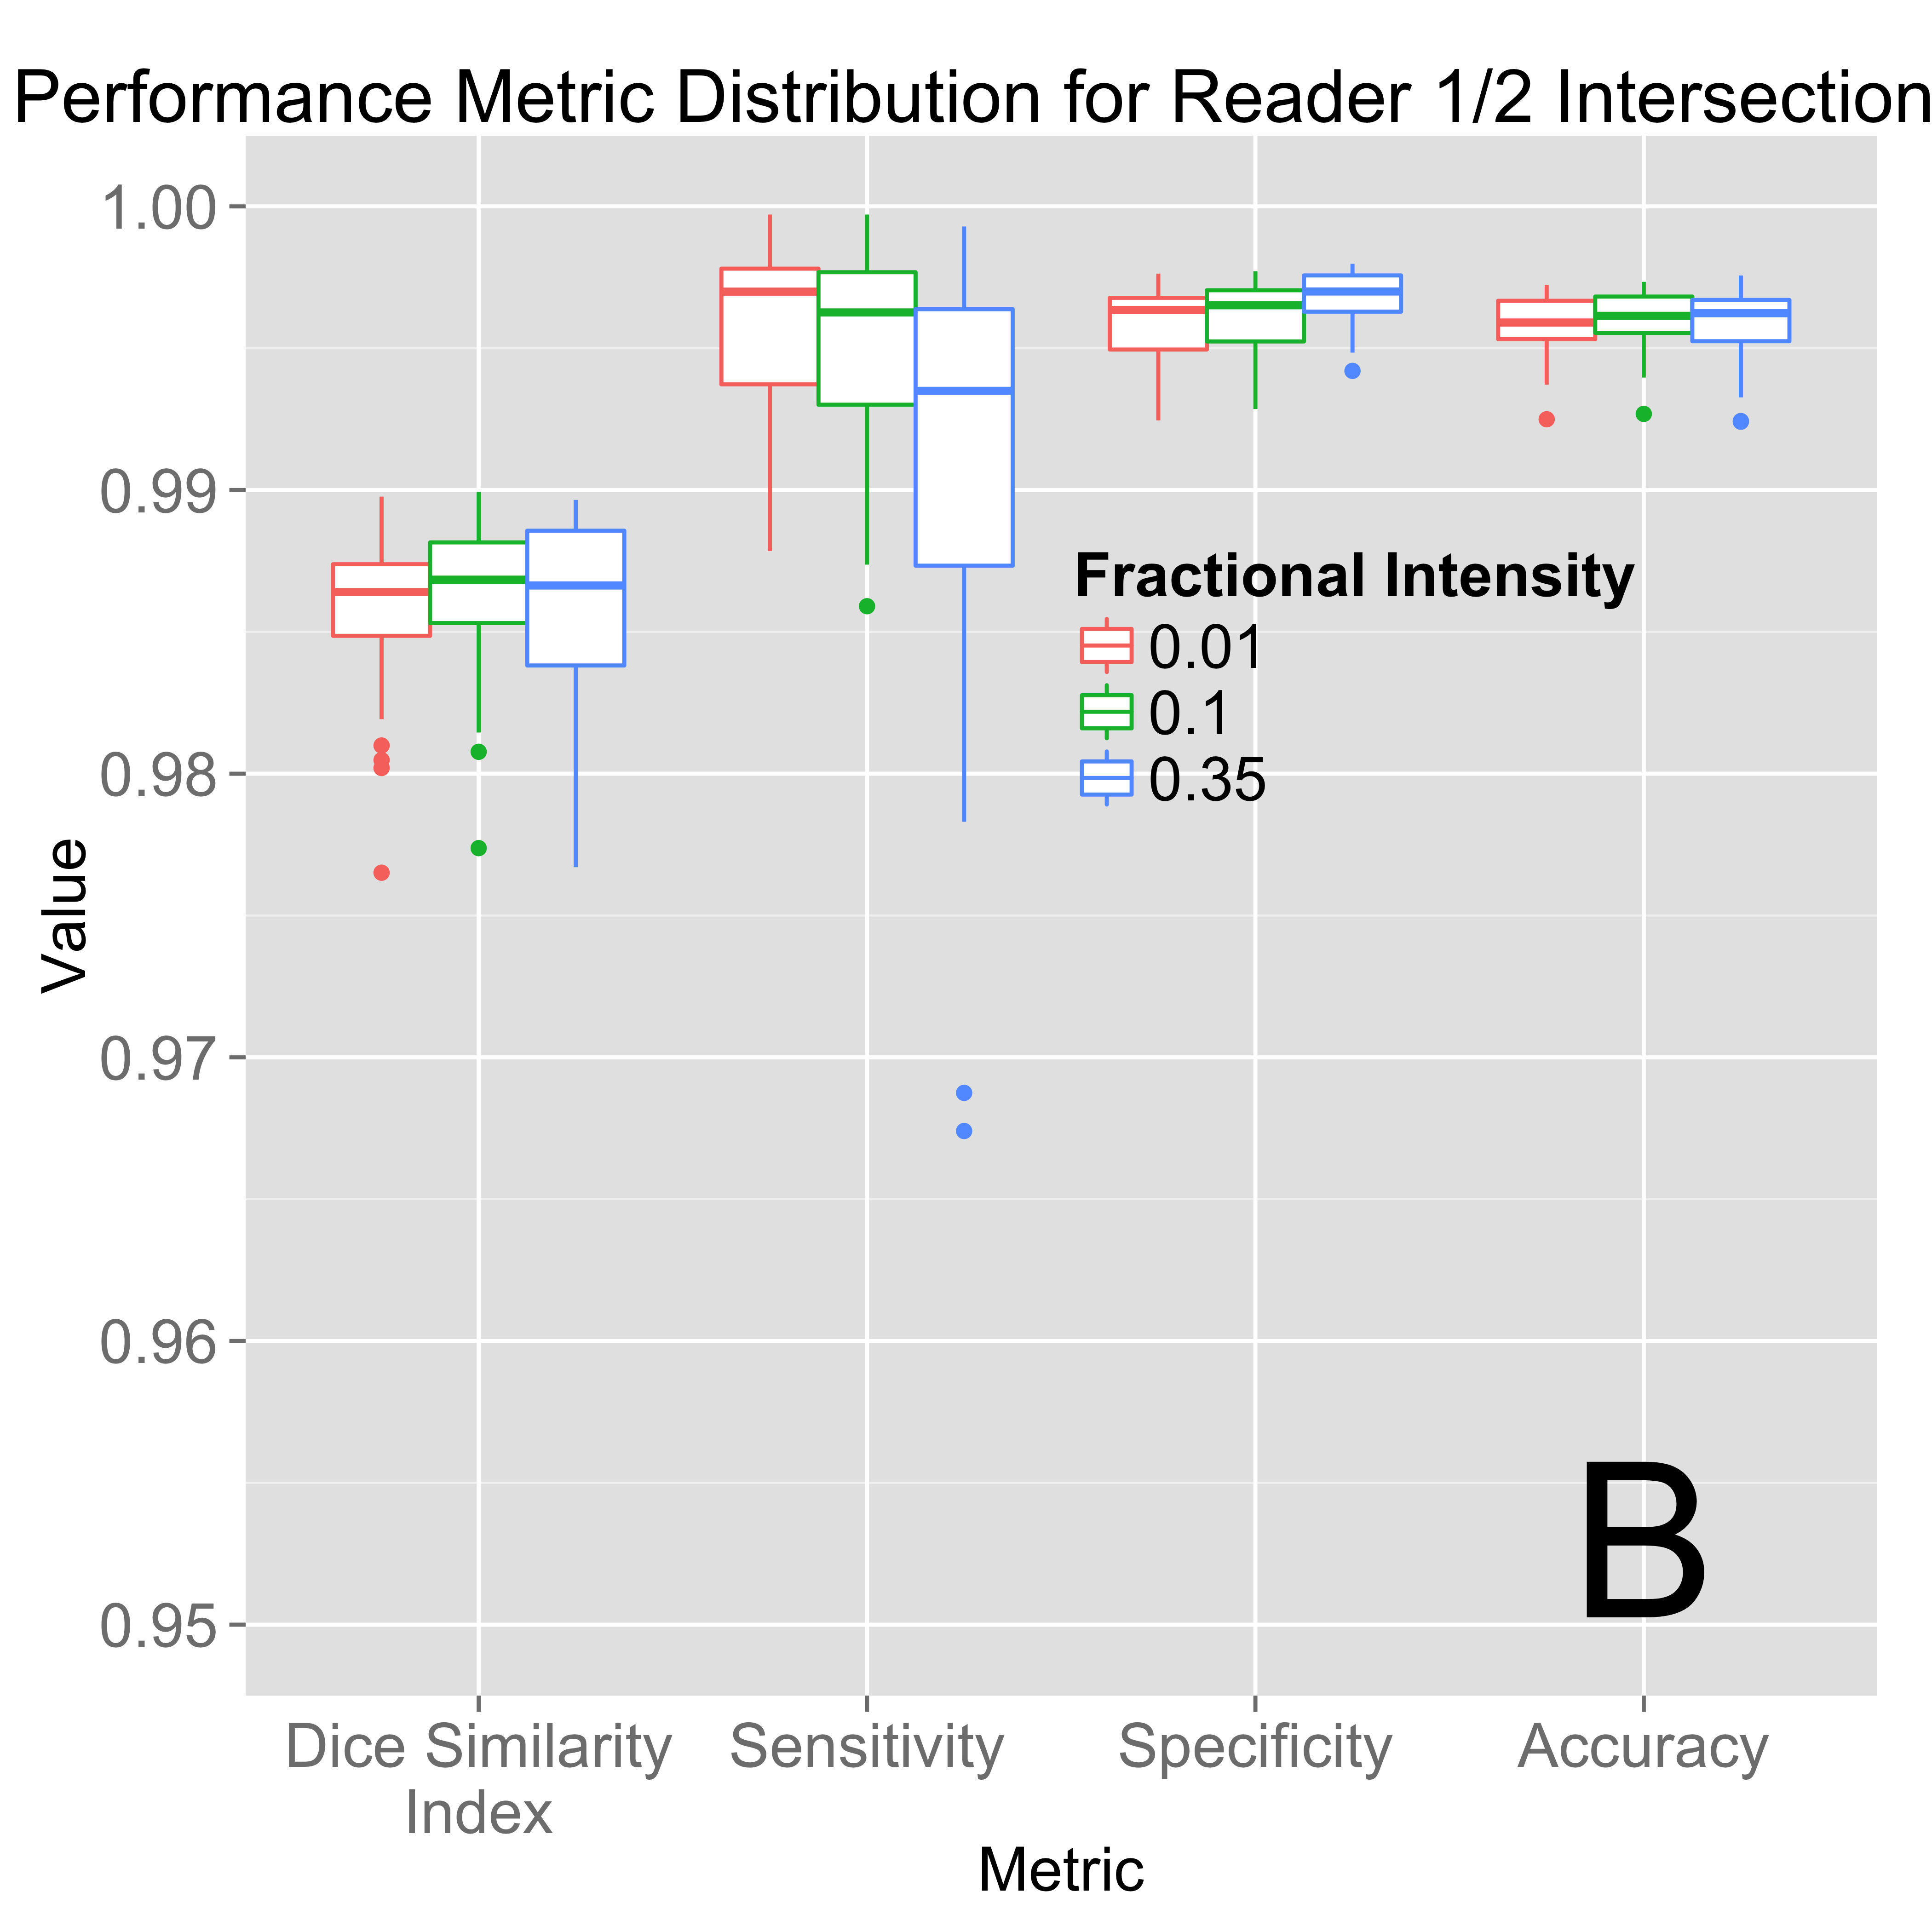
\includegraphics[width=.315\textwidth]{figure/Intersection_CT_Skull_Stripping_Figure2b.png}
}
\hfill
  \subfloat{
  \label{union}
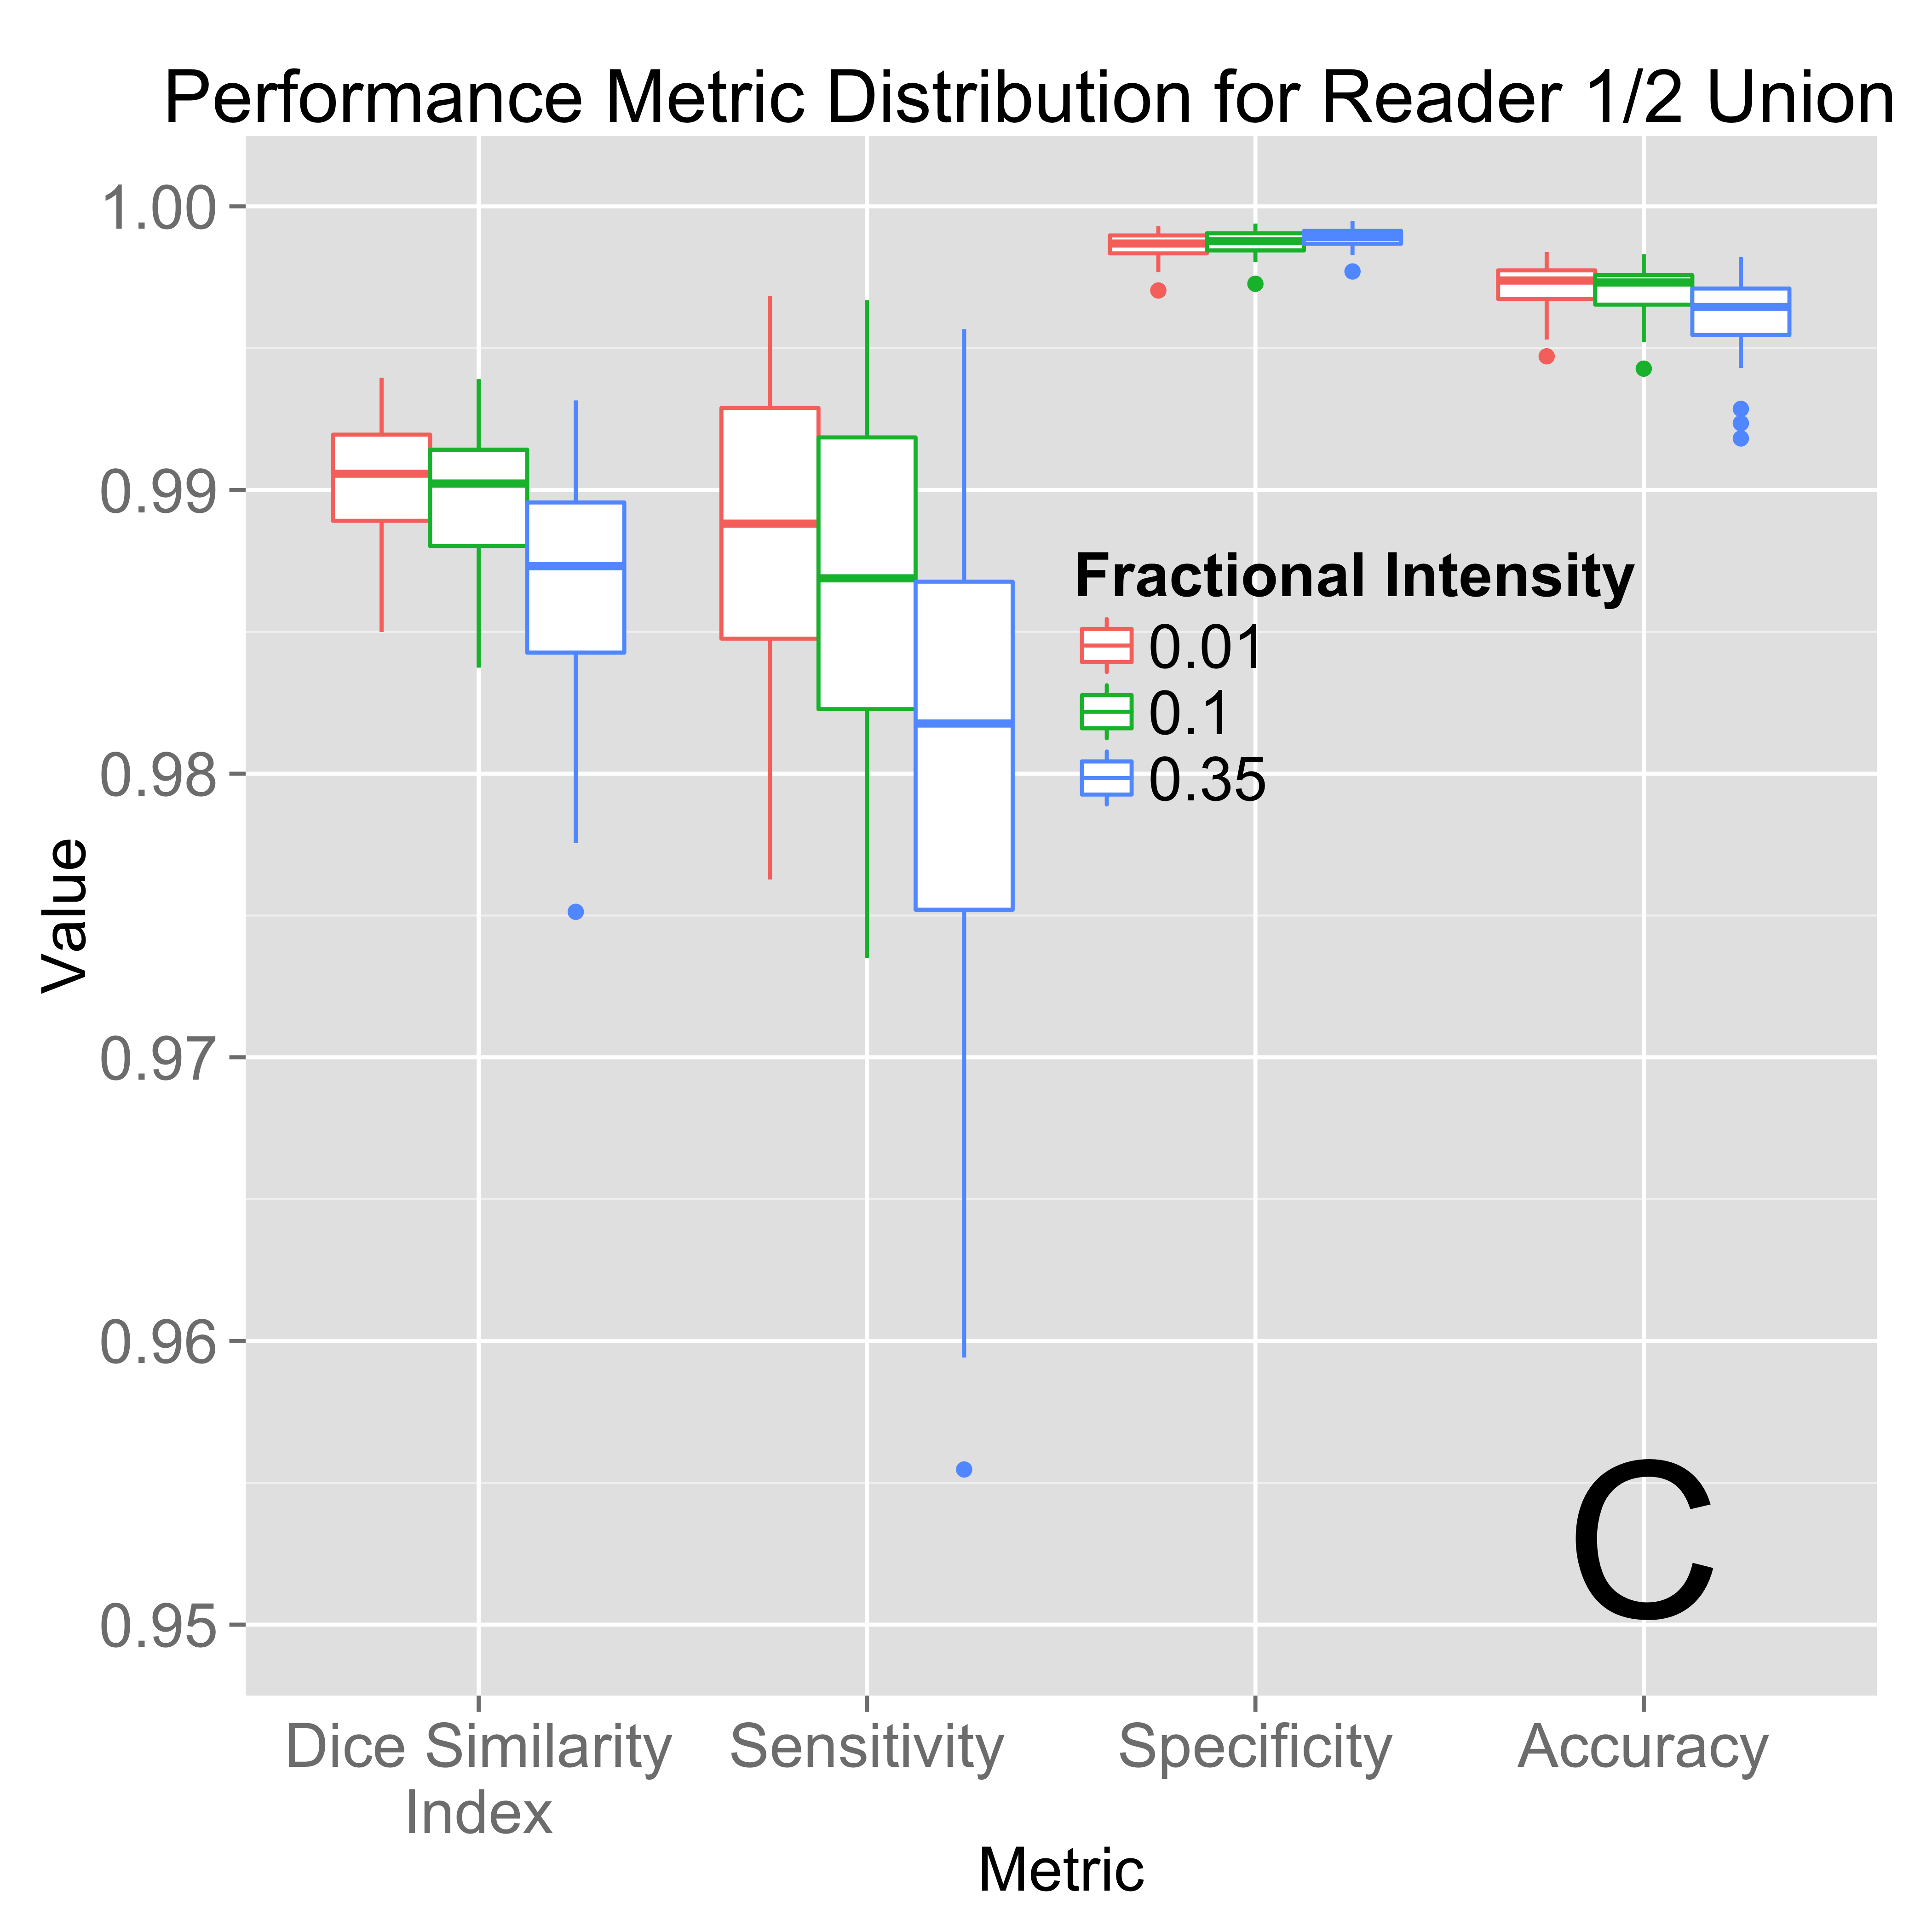
\includegraphics[width=.315\textwidth]{figure/Union_CT_Skull_Stripping_Figure2b.png}
}
\caption[{\bf Comparison of Performance Measures from 2 Manual Brain Segmentations.}]{We display the boxplots for performance measures of the automated segmentation when using smoothed data with different fractional intensity (FI) with the gold standard being the manual segmentation from reader 2 \protect\subref{reader2}, scan-wise intersection of the manual segmentation from reader 1 and reader 2~\protect\subref{intersect}, or scan-wise union of the manual segmentation from reader 1 and reader 2~\protect\subref{union}.  Overall, using an FI of $0.01$ and $0.1$ perform high on all measures, regardless of manual segmentation used as the gold standard. }
\label{fig:union_intersect}
\end{figure}

\section*{Inline Supplementary Figure 2}
\begin{figure}[H]
  \subfloat{
  \label{corrplot}
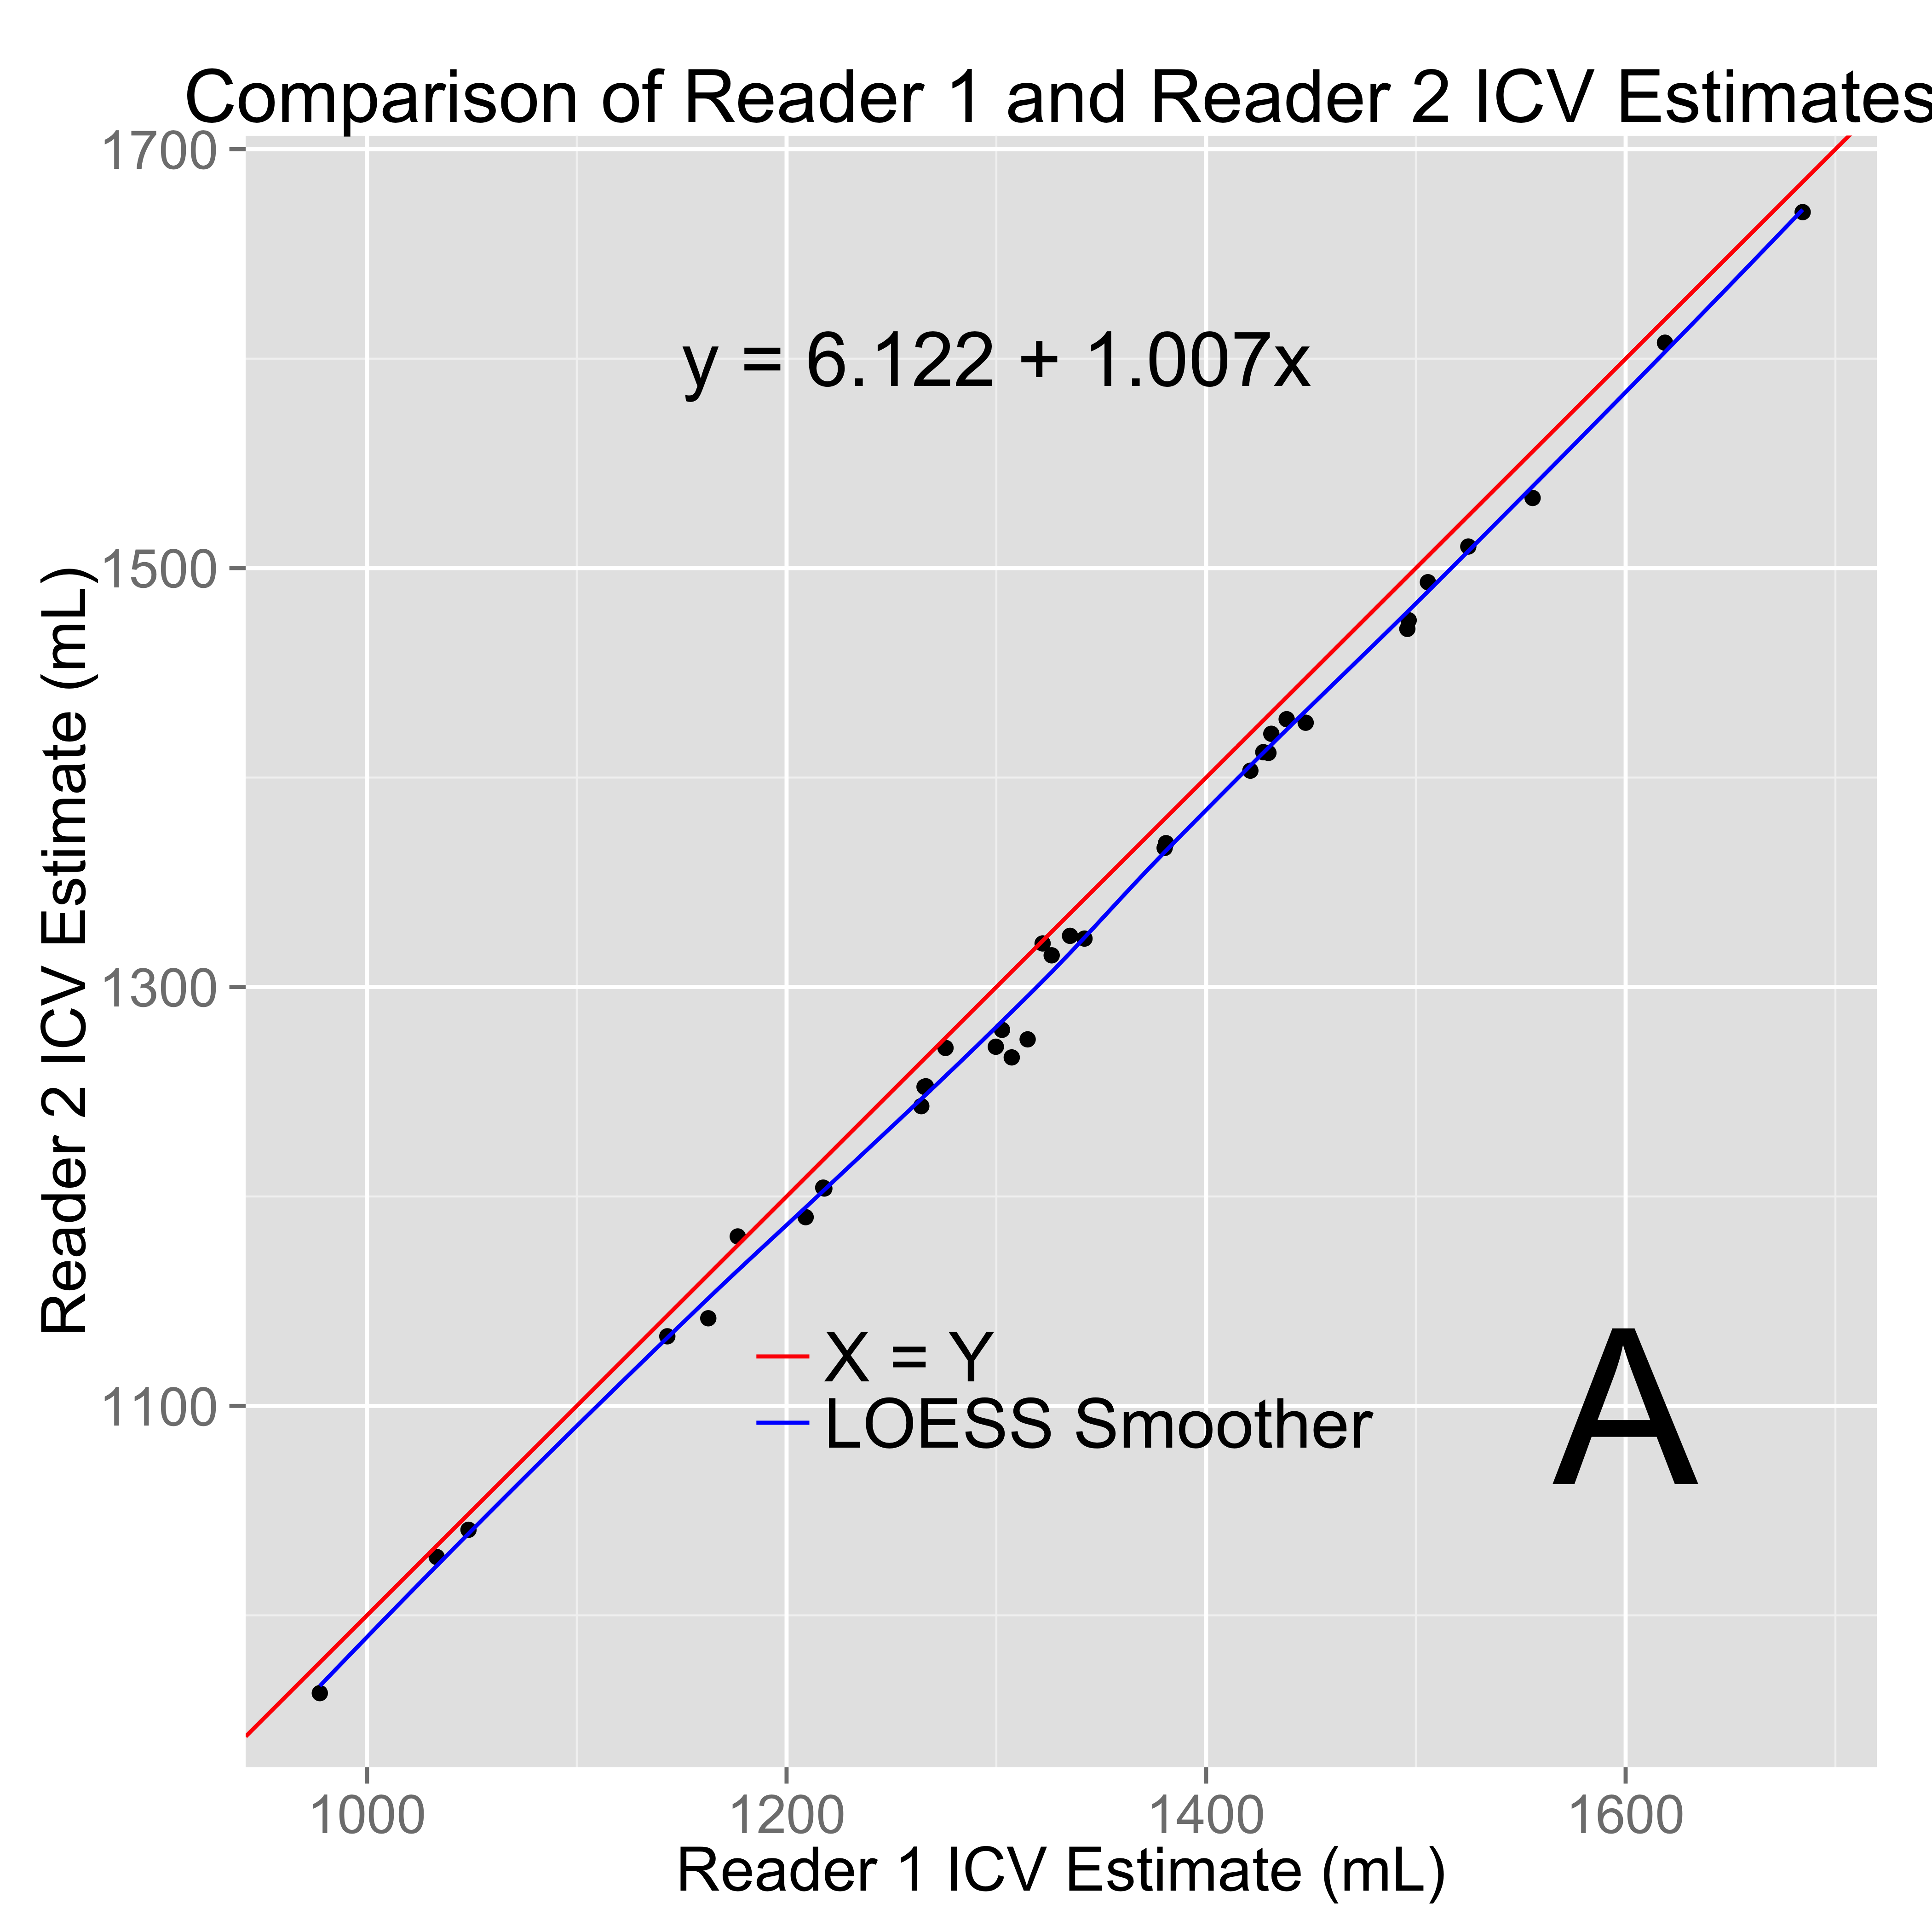
\includegraphics[width=.48\textwidth]{figure/Corr_Plot_Readers.png}
}
\hfill
  \subfloat{
  \label{baplot}
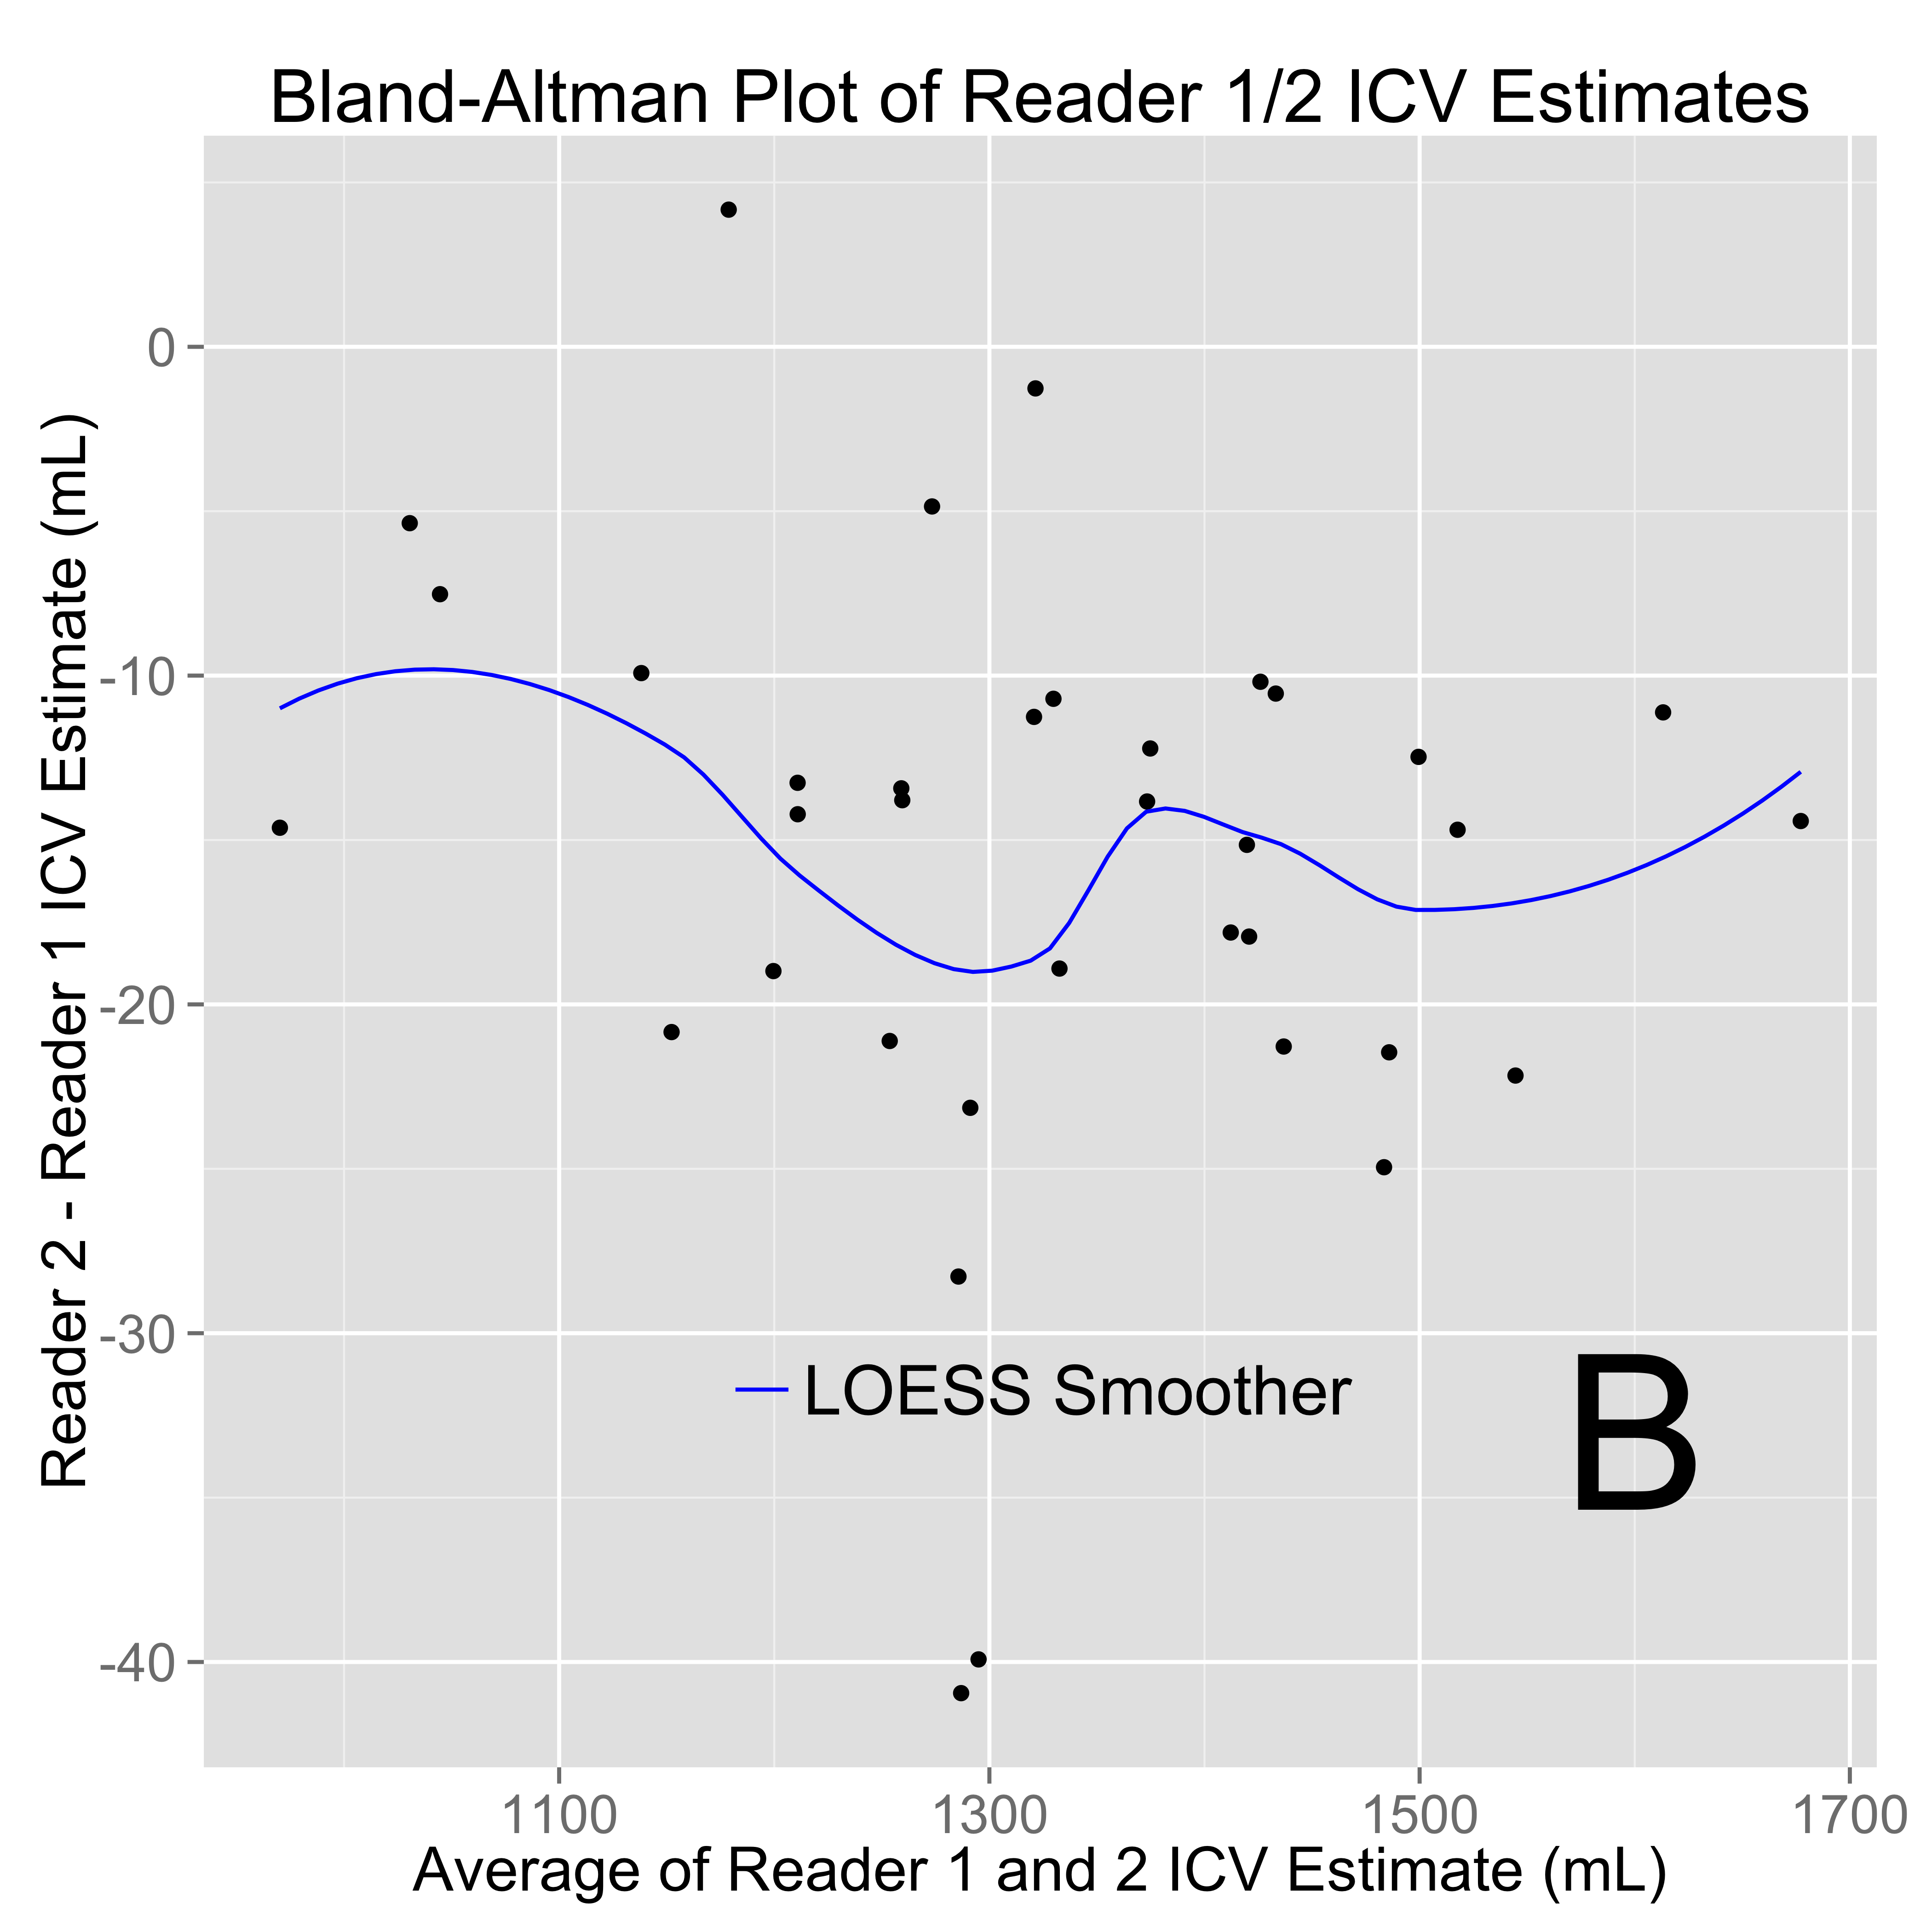
\includegraphics[width=.48\textwidth]{figure/BA_Plot_Readers.png}
}
\caption[{\bf Comparison of Intracranial Volume (ICV) Estimates from 2 Manual Brain Segmentations.}]{ Panel~\protect\subref*{corrplot} displays the intracranial volume (ICV) estimate from the manual segmentation of reader 1 versus reader 2.  The blue line represents a LOESS scatterplot smoother of the data.  The red line represents a linear fit.  The slope is approximately 1 and the intercept is approximately 6 mL, indicating strong agreement of the estimates.  The Bland-Altman plot in panel~\protect\subref*{baplot} denotes that there is no strong effect of the size of segmentation on the difference, but the ICV of reader 1 is higher on average than that of reader 2.  These differences are small compared to the value of the ICV estimate, however.}
\label{fig:reader_compare}
\end{figure}


